\documentclass[14pt,xcolor=dvipsnames,table,dvipdfmx]{beamer}

\setbeamertemplate{bibliography item}[text]
\usepackage[absolute,overlay]{textpos}
\usepackage{apalike}
\usetheme{Boadilla}

\usepackage{txfonts} % TXフォント
\renewcommand{\kanjifamilydefault}{\gtdefault}  % 日本語をゴシック体に
\usefonttheme{structurebold} % タイトル部を太字
\setbeamerfont{alerted text}{series=\bfseries} % Alertを太字
\setbeamerfont{section in toc}{series=\mdseries} % 目次は太字にしない
\setbeamerfont{frametitle}{size=\Large} % フレームタイトル文字サイズ
\setbeamerfont{title}{size=\LARGE} % タイトル文字サイズ
\setbeamerfont{date}{size=\small}  % 日付文字サイズ
\usepackage{pxjahyper}

\uselanguage{japanese}
\languagepath{japanese}
\deftranslation[to=japanese]{Theorem}{定理}
\deftranslation[to=japanese]{Lemma}{補題}
\deftranslation[to=japanese]{Example}{例}
\deftranslation[to=japanese]{Examples}{例}
\deftranslation[to=japanese]{Definition}{定義}
\deftranslation[to=japanese]{Definitions}{定義}
\deftranslation[to=japanese]{Problem}{問題}
\deftranslation[to=japanese]{Solution}{解}
\deftranslation[to=japanese]{Fact}{事実}
\deftranslation[to=japanese]{Proof}{証明}
\def\proofname{証明}

\definecolor{UniBlue}{RGB}{0,150,200} 
\definecolor{AlertOrange}{RGB}{255,76,0}
\definecolor{AlmostBlack}{RGB}{38,38,38}
\setbeamercolor{normal text}{fg=AlmostBlack}  % 本文カラー
\setbeamercolor{structure}{fg=UniBlue} % 見出しカラー
\setbeamercolor{block title}{fg=UniBlue!50!black} % ブロック部分タイトルカラー
\setbeamercolor{alerted text}{fg=AlertOrange} % \alert 文字カラー
\mode<beamer>{
    \definecolor{BackGroundGray}{RGB}{254,254,254}
    \setbeamercolor{background canvas}{bg=BackGroundGray} % スライドモードのみ背景をわずかにグレーにする
}

% Algorithm系
\usepackage{algorithm}
\usepackage[noend]{algorithmic}
\algsetup{linenosize=\color{fg!50}\footnotesize}
\renewcommand\algorithmicdo{:}
\renewcommand\algorithmicthen{:}
\renewcommand\algorithmicrequire{\textbf{Input:}}
\renewcommand\algorithmicensure{\textbf{Output:}}

%フラットデザイン化
\setbeamertemplate{blocks}[rounded] % Blockの影を消す
\useinnertheme{circles} % 箇条書きをシンプルに
\setbeamertemplate{navigation symbols}{} % ナビゲーションシンボルを消す
\setbeamertemplate{footline}[frame number] % フッターはスライド番号のみ

\AtBeginSection[]{
    \frame{\tableofcontents[currentsection, hideallsubsections]} %目次スライド
}

\newcommand{\tabincell}[2]{\begin{tabular}{@{}#1@{}}#2\end{tabular}}

\title{\bfseries プライバシーを保護する特許検索}

\date{2016年月日}
\author{中川研M2 胡 瀚林 \\ 指導教員:中川 裕志 教授}
%\subject{PIR}
%\keywords{PIR,Obfuscation,query}

\begin{document}

\maketitle
\frame{\tableofcontents[hideallsubsections]}

\section{背景紹介}
\begin{frame}{特許}
	\begin{block}{特許とは?}
		\begin{itemize}
        \item 特許法第1条には、「この法律は、発明の保護及び利用を図ることにより、発明を奨励し、もつて産業の発達に寄与することを目的とする」とある。
		\item 特許制度は、発明者には一定期間、一定の条件のもとに特許権という独占的な権利を与えて発明の保護を図る一方、その発明を公開して利用を図ることにより新しい技術を人類共通の財産としていくことを定めて、これにより技術の進歩を促進し、産業の発達に寄与しようというものである。
		\end{itemize}
	\end{block}
\end{frame}

\begin{frame}{特許}
    \begin{exampleblock}{特許請求の範囲}
		【請求項1】植物の種子をパルプ繊維の水懸濁液に混合して抄紙する播種シートの製造方法。\\
		【請求項2】水懸濁液にさらに水溶性接着剤を添加する請求項1記載の播種シートの製造方法。\\
		【請求項3】あらかじめ種子を低粘度多価アルコールで被覆する請求項1記載の播種シートの製造方法。
    \end{exampleblock}
	\begin{block}{特許請求の範囲の作成方法}
		8技術用語は、学術用語を用いる。\\
		9用語は、その有する普通の意味で使用し、かつ、明細書及び特許請求の範囲全体を通じて統一して使用する	
	\end{block}
\end{frame}


\begin{frame}{特許検索}
	\begin{block}{}
		\fontsize{8pt}{7.2}\selectfont
		\begin{tabular}{ccc}
        \noalign{\hrule height 1pt}
        検索タイプー & 検索対象(specification) & 検索目的 \\
        \hline
        \tabincell{c}{技術水準調査\\(State of the Art Search)} & イデア & 自分の発明に関連する背景知識を得る \\
        \tabincell{c}{新規性調査\\(Novelty Search)} & 特許文章 & 特許登録の可能性を判断する \\
        \tabincell{c}{侵害調査\\(Infringement Search)} &  \tabincell{c}{商品と\\商品に関連する技術} & 権利侵害とならないかを判断する \\
        \noalign{\hrule height 1pt}
        \end{tabular}
	\end{block}
\end{frame}

\begin{frame}{新規性調査}
\begin{columns}[t]
    \begin{column}{0.8\textwidth} % 横幅の30%
      	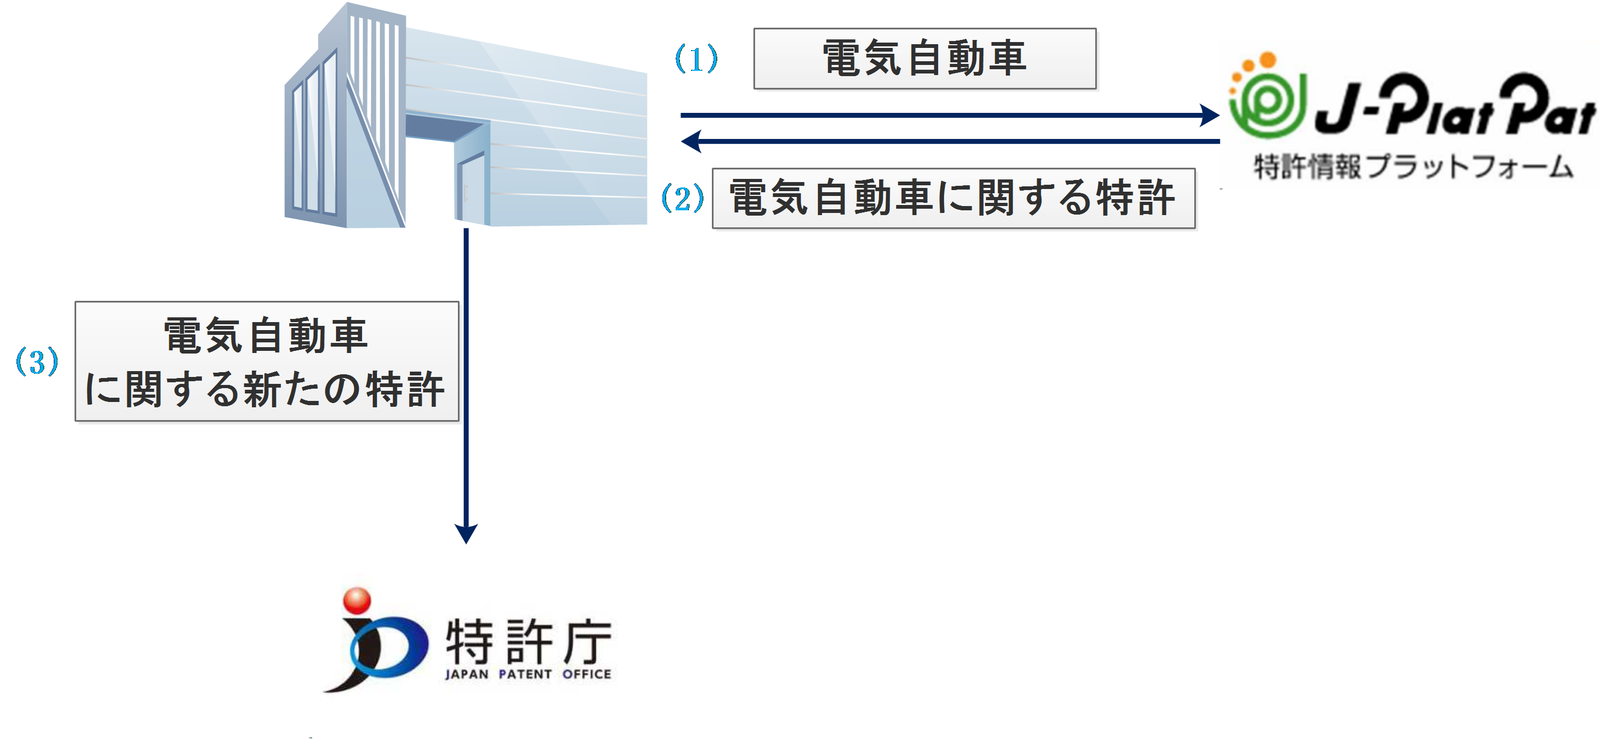
\includegraphics[width=\columnwidth]{rk1.png}
    \end{column}
\end{columns}
\end{frame}

\begin{frame}{新規性調査}
\begin{columns}[t]
    \begin{column}{0.8\textwidth} % 横幅の30%
      	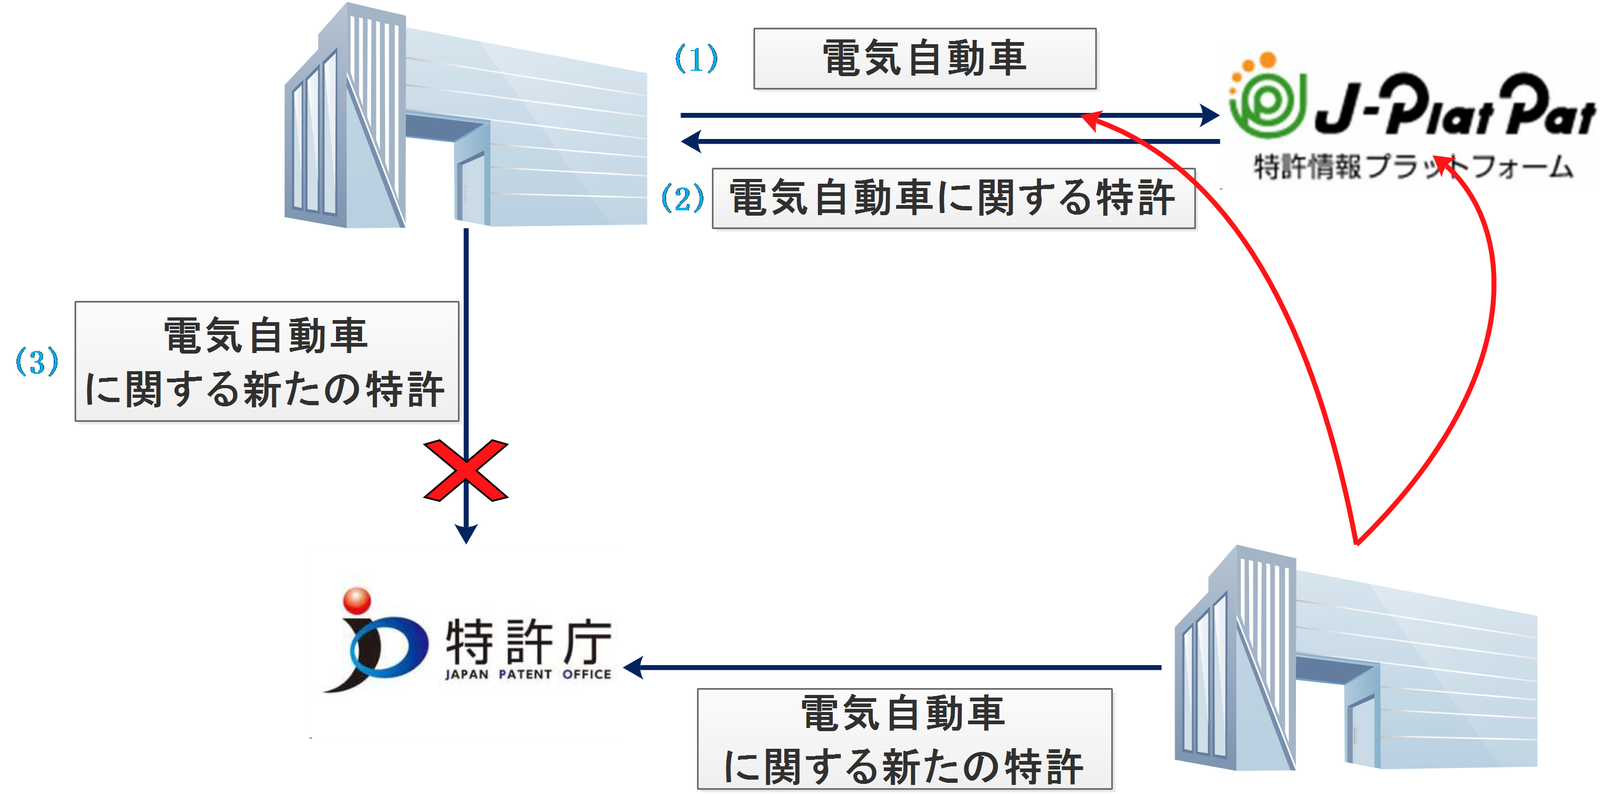
\includegraphics[width=\columnwidth]{rk2.png}
    \end{column}
\end{columns}
\end{frame}

\begin{frame}{特許検索質問}
	\fontsize{10pt}{7.2}\selectfont
	\begin{exampleblock}{播種シートの製造方法}
		植物 種子 パルプ 繊維 水 液 混合 抄 紙 播種 シート 製造 方法 水溶 性 接着 剤 添加 記載 度 価 アルコール 被覆
	\end{exampleblock}
	\fontsize{14pt}{7.2}\selectfont
	\begin{block}{}
    \begin{itemize}
        \item 検索質問は単語(名詞)の集合である
        \item 質問に含む単語数が多い
		\begin{itemize}
			\item ウェブ検索:2.35 特許検索:20.1
		\end{itemize}
		\item 専門用語が多い
    \end{itemize}
	\end{block}
\end{frame}

\begin{frame}{テキスト検索}
\begin{columns}[t]
    \begin{column}{0.8\textwidth} % 横幅の30%
        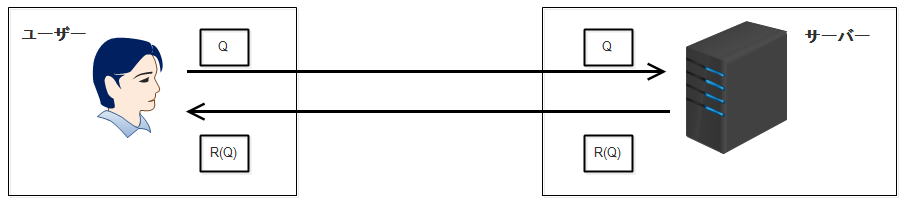
\includegraphics[width=\columnwidth]{photo1.png}
    \end{column}
\end{columns}
    \begin{block}{}
    \begin{itemize}
        \item 検索質問$Q$:単語の集合
        \item 質問$Q$の検索結果$R(Q)$:文章の集合
    \end{itemize}
    \end{block}
\end{frame}

\begin{frame}{Obfuscation Search}
    \begin{columns}[t]
        \begin{column}{1\textwidth} % 横幅の30%
            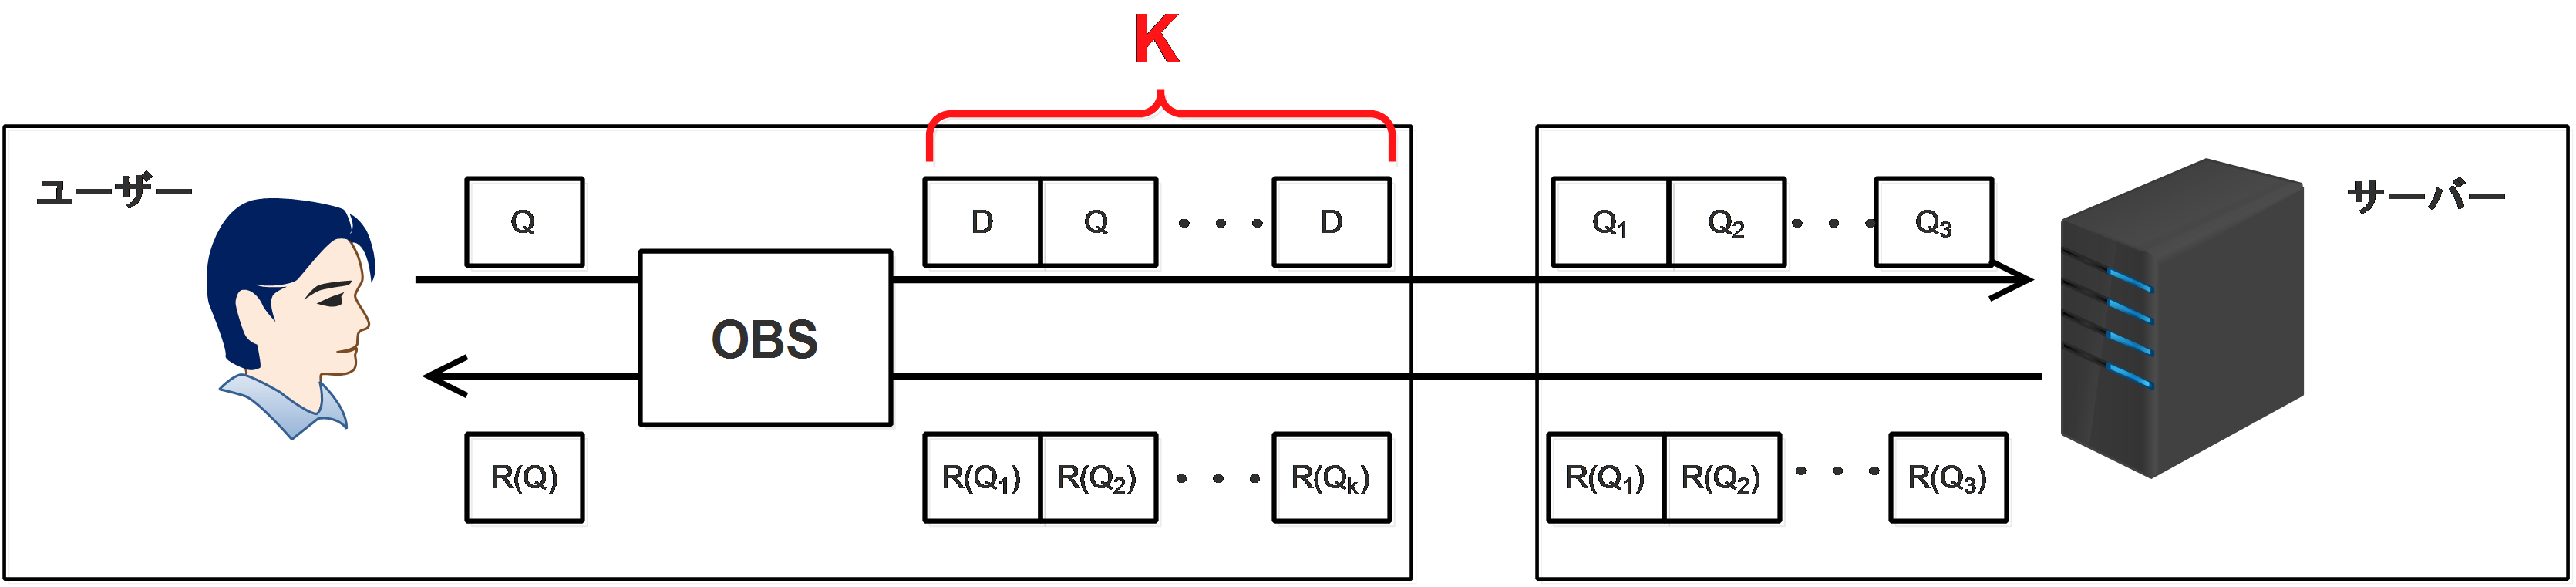
\includegraphics[width=\columnwidth]{rk4.png}
		\end{column}
    \end{columns}
	\begin{block}{} 
		\begin{itemize}
			\item 真の質問と$K-1$個真の質問と区別できないダミー質問と同時に検索する
			\item サーバーが真の質問を見つける確率が$1/k$
		\end{itemize}
	\end{block}
\end{frame}

\begin{frame}{Obfuscation Search:例}
    \begin{columns}[t]
        \begin{column}{1\textwidth} % 横幅の30%
            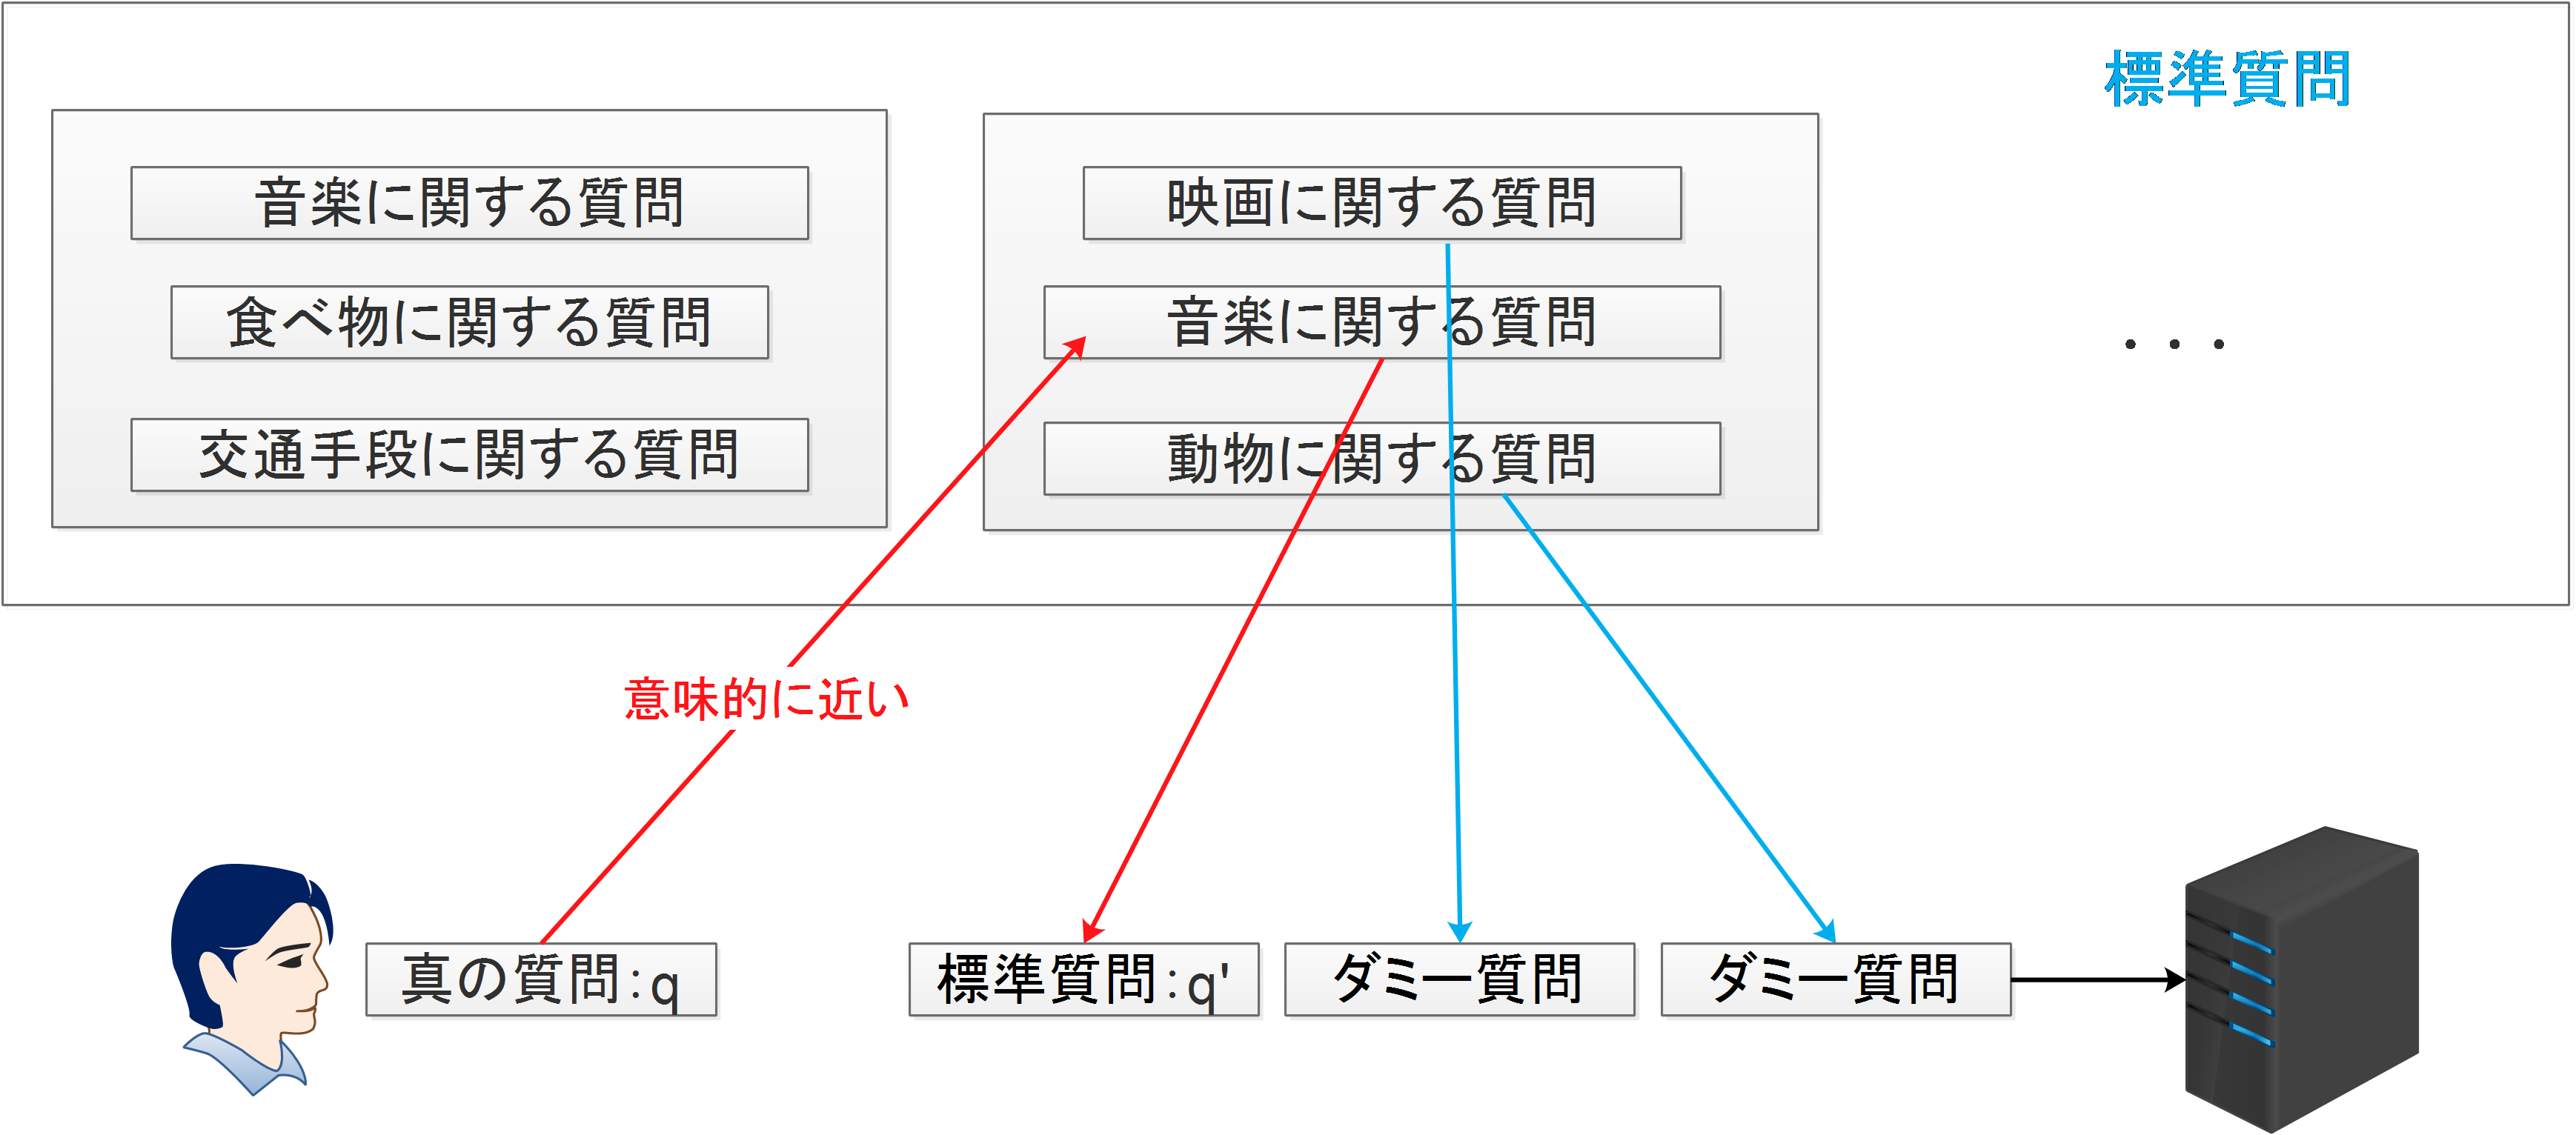
\includegraphics[width=\columnwidth]{rk14.png}
		\end{column}
    \end{columns}
	\begin{block}{} 
		\begin{itemize}
			\item 実践的には長い質問に対応できない
			\item 質問$q'$を使うことより検索の精度と再現率が下がる
		\end{itemize}
	\end{block}
\end{frame}

\begin{frame}{目標}
    \begin{block}{}
    \begin{itemize}
        \item 長い質問に対応できる
        \item 専門用語が多いダミーを生成できる
		\item 検索の精度と再現率を維持できる
    \end{itemize}
    \end{block}
\end{frame}

\section{既存研究}
\begin{frame}{Embellishing Text Search Queries to Protect User Privacy \cite{pang_embellishing_2010}}
	\begin{columns}[t]
		\begin{column}{0.8\textwidth} % 横幅の30%
			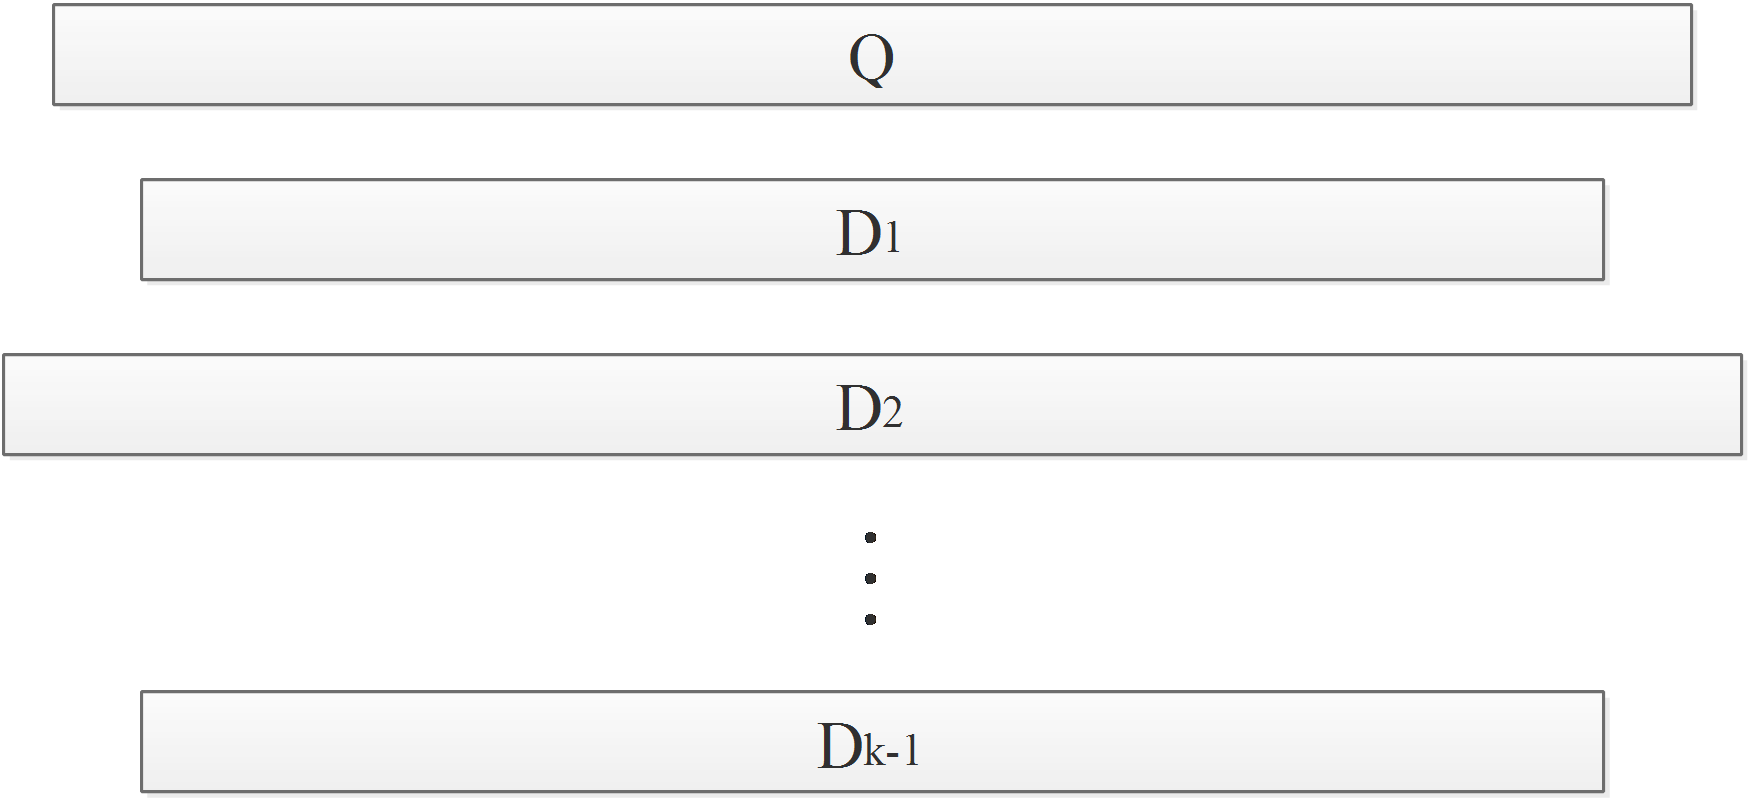
\includegraphics[width=\columnwidth]{rk6.png}
		\end{column}
	\end{columns}
	\begin{block}{}
		真の質問である可能性がある質問数:$K$	
	\end{block}
\end{frame}

\begin{frame}{ETS}
	\begin{columns}[t]
		\begin{column}{0.8\textwidth} % 横幅の30%
			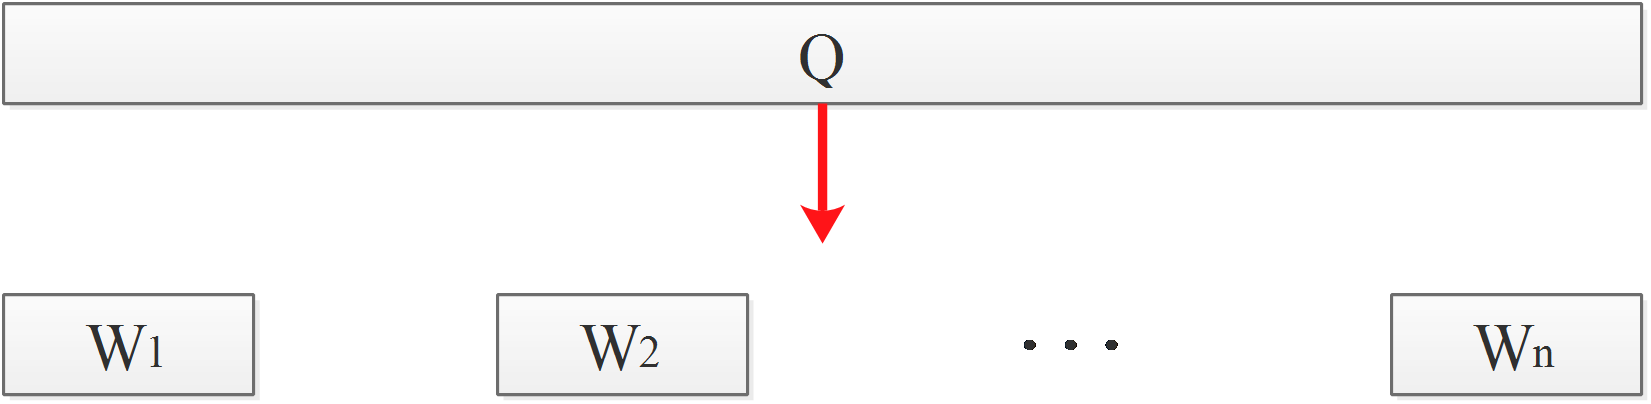
\includegraphics[width=\columnwidth]{rk7.png}
		\end{column}
	\end{columns}
\end{frame}

\begin{frame}{ETS}
	\begin{columns}[t]
		\begin{column}{0.8\textwidth} % 横幅の30%
			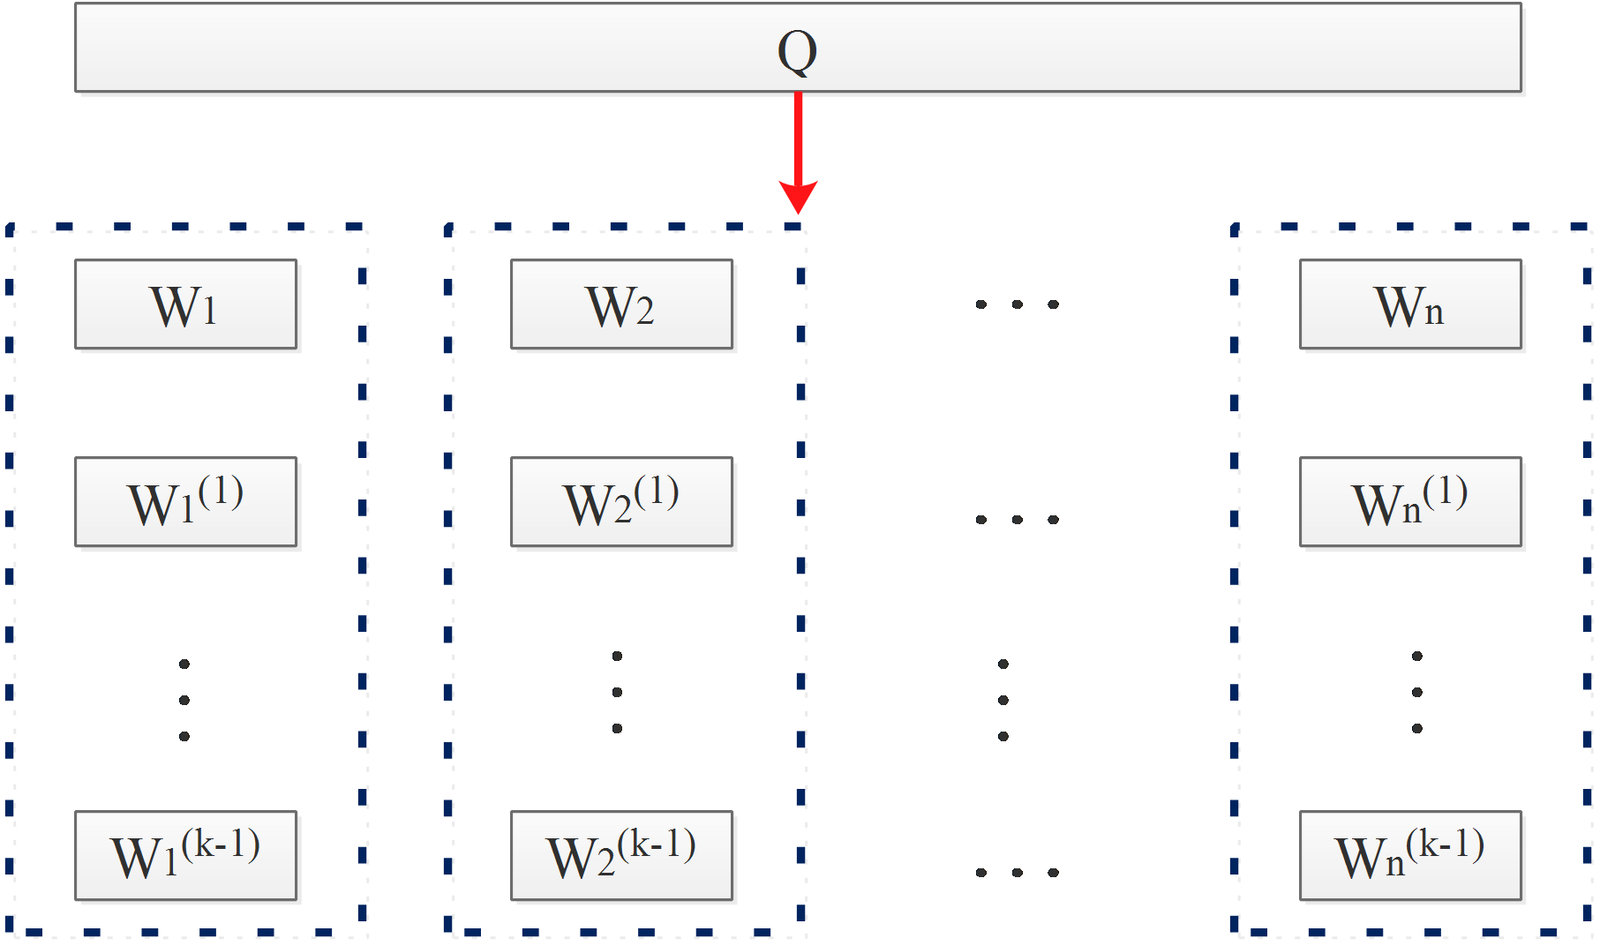
\includegraphics[width=\columnwidth]{rk8.png}
		\end{column}
	\end{columns}
	\begin{block}{}
		真の質問である可能性がある質問数:$K \textcolor{red}\rightarrow K^n$	
	\end{block}
\end{frame}

\begin{frame}{テキスト検索}
\fontsize{12pt}{7.2}\selectfont
		\center
		\begin{tabular}{|c|c|}
		\noalign{\hrule height 1pt}
		単語 & 文章id \\
		\hline
		モーツァルト & $1,3$\\
		交響曲 & $1,2,3$ \\
		パン & $2,4$ \\
		飛行機 & $4$ \\
		\noalign{\hrule height 1pt}
		\end{tabular}\\
		\center
		転置フィル
	\begin{block}{}
	ユーザー質問:モーツァルト 交響曲 \\
	検索結果:$R = \{1,3\} \cup \{1,2,3\} = \{1,3\}$
	\end{block}
\end{frame}

\begin{frame}{テキスト検索}
\fontsize{12pt}{7.2}\selectfont
		\center
		\begin{tabular}{|c|c|}
		\noalign{\hrule height 1pt}
		単語 & $\langle$文章id,単語と文章の関係値$\rangle$ \\
		\hline
		モーツァルト & $\langle1,1\rangle,\langle3,2\rangle$\\
		交響曲 & $\langle1,1\rangle,\langle2,3\rangle,\langle3,2\rangle$ \\
		パン & $\langle2,1\rangle,\langle4,1\rangle$ \\
		飛行機 & $\langle4,2\rangle$ \\
		\noalign{\hrule height 1pt}
		\end{tabular}\\
		\center
		転置フィル
	\begin{block}{}
	ユーザー質問:モーツァルト 交響曲 \\
	
	質問単語の転置リストに存在する各文章の関係値を計算する:\\
	$\{ \langle1,1+1\rangle,\langle2,3\rangle,\langle3,2+2\rangle \} = \{ \langle1,2\rangle,\langle2,3\rangle,\langle3,4\rangle \}$\\
	関係値により並び替える:$R = \{ 3,2,1 \}$
	\end{block}
\end{frame}

\begin{frame}{テキスト検索}
\fontsize{12pt}{7.2}\selectfont
	\begin{columns}[t]
		\begin{column}{0.8\textwidth} % 横幅の30%
			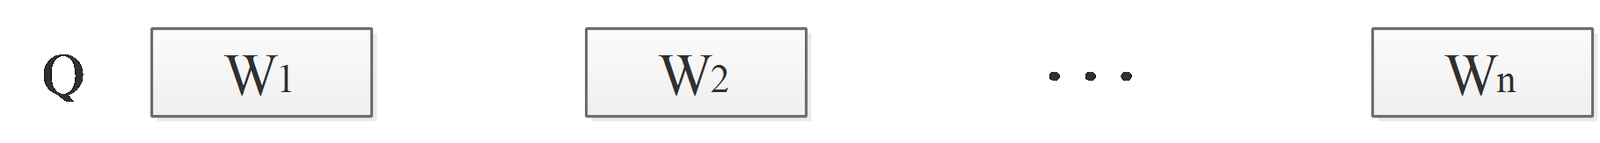
\includegraphics[width=\columnwidth]{rk9.png}
		\end{column}
	\end{columns}
	\begin{block}{}
		単語$W_i$に対して文章$d_j$のスコア:$s_{ij}$ \\
		質問$Q$に対して文章$d_j$のスコア:$s_{j}=\sum_{i \in Q}s_{ij}$ \\
		スコアが上位$m$個にある文章を質問$Q$の検索結果として返す
	\end{block}
\end{frame}

\begin{frame}{凖同型暗号}
	\begin{Definition}[凖同型暗号]
		二つの暗号文 $Enc(m_1), Enc (m_2)$ が与えられた時に、平文や秘密鍵なしで $Enc( m_1 \circ m_2 )$ を計算できる暗号
	\end{Definition}
	\begin{Example}[加算ができる凖同型暗号]
		$E(\cdot):$ 暗号化 \, $D(\cdot):$復号 \\
		\begin{itemize}
			\item ランダム性:$E(m) \neq E(m)$
			\item $ E(m_1) \cdot E (m_2) = E(m_1 + m_2) $
			\item $ E(m)^q = E(m \cdot q) , \, q \in \mathbb{Z}^+$
		\end{itemize}
	\end{Example}
\end{frame}

\begin{frame}{質問検索-ETS}
\fontsize{12pt}{7.2}\selectfont
	\begin{minipage}[c]{0.65\textwidth}
			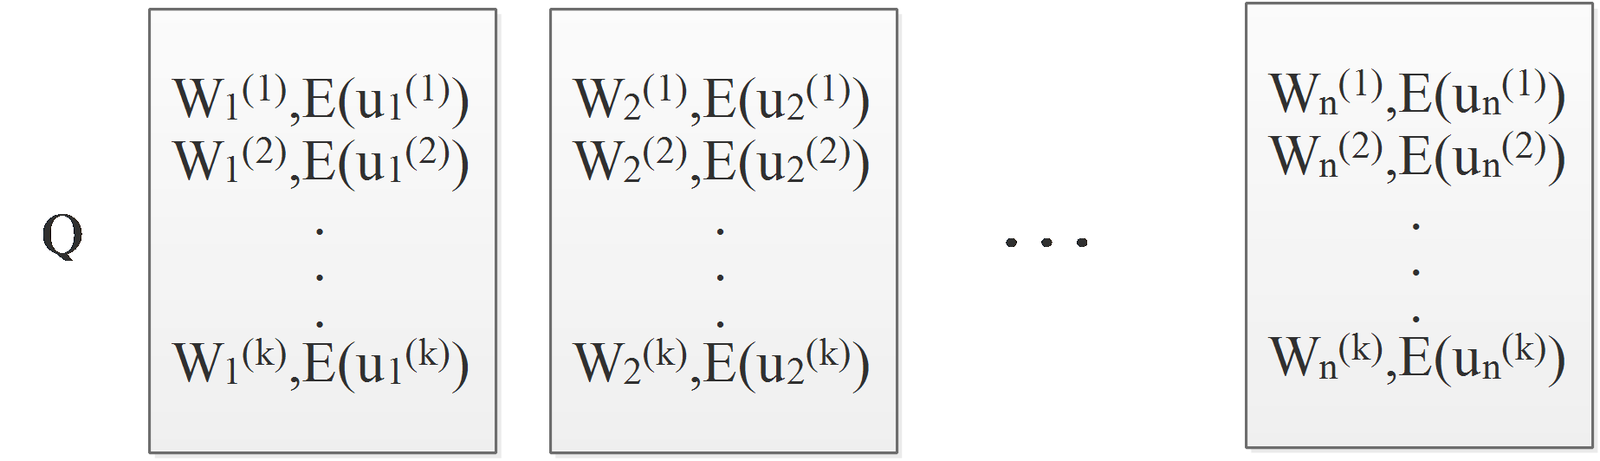
\includegraphics[width=\columnwidth]{rk10.png}
	\end{minipage}%
	\begin{minipage}[c]{0.25\textwidth}
			$$\,\,u_i^{(k)}=\left\{
			\begin{aligned}
			0& \, i,k \notin Q^* \\
			1& \, i,k \in Q^*
			\end{aligned}
			\right.
			$$
	\end{minipage}
	\begin{block}{}
		単語$W_i^{(k)}$に対して文章$d_j$のスコア:$s'_{ikj}=E(u_i^{(k)})^{(s_{ikj})}=E(u_i \cdot (s_{ikj}))$ \\
		質問$Q$に対して文章$d_j$のスコア:$s_{j}=\prod_{i,k \in Q}s'_{ikj}=E(\sum_{i,k \in Q^*}s_{ikj})$ \\
		スコアが$0$ではない文章を全部返す
	\end{block}
\end{frame}

\begin{frame}{質問検索-ETS}
	\begin{exampleblock}{}
      		 \begin{columns}[c]
           		\begin{column}{0.3\textwidth} % 横幅の30%
               		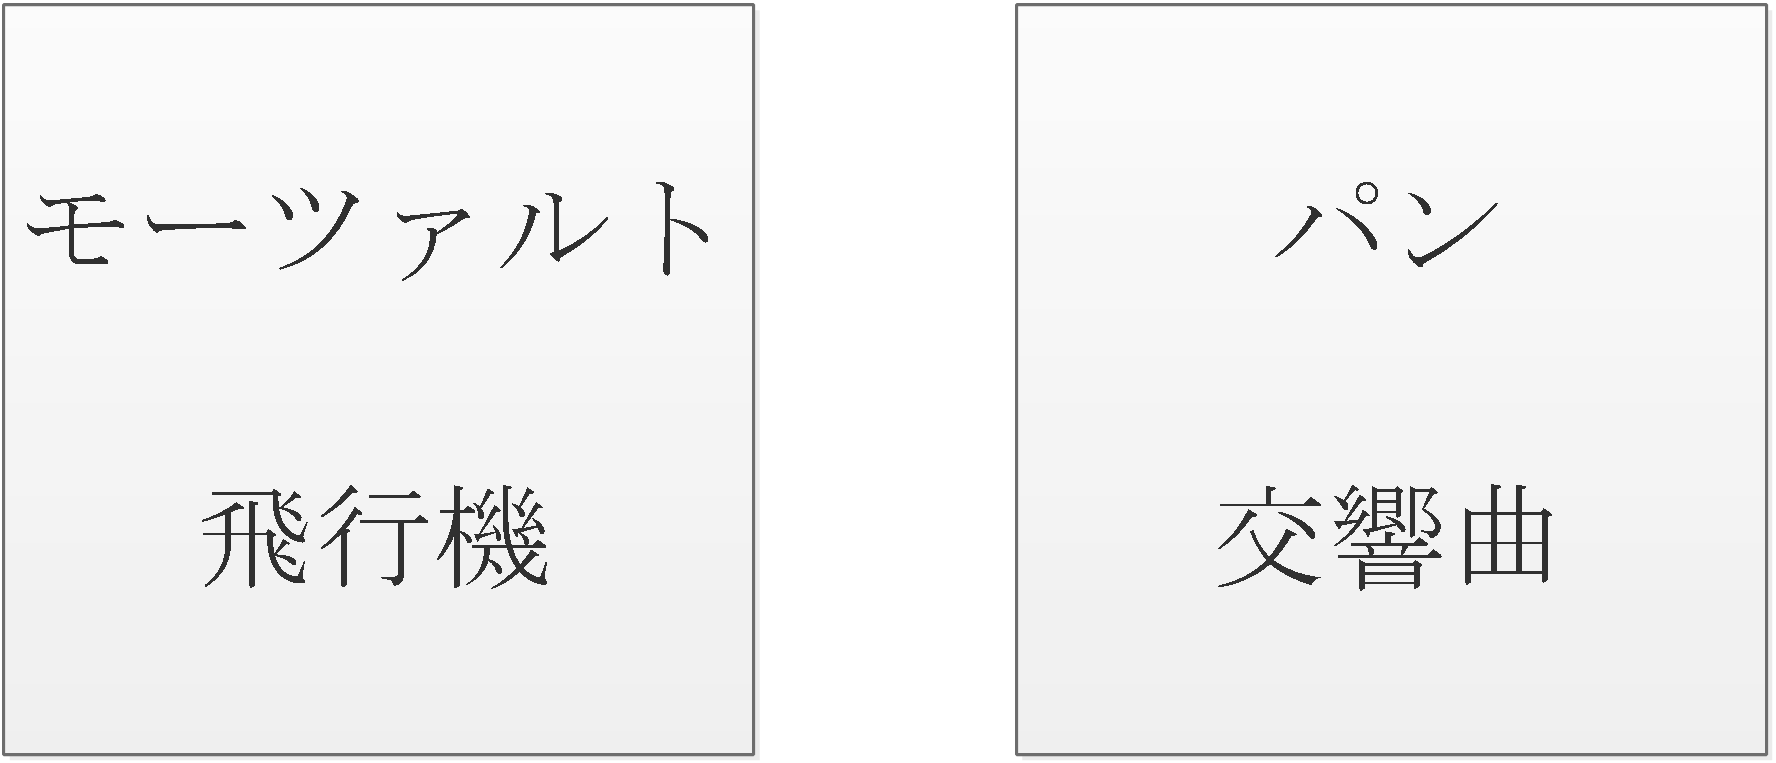
\includegraphics[width=\columnwidth]{rk16.png}
		   	\end{column}
       		\begin{column}{0.68\textwidth} % 横幅の30%
\fontsize{9pt}{7.2}\selectfont
				\begin{tabular}{|c|c|}
				\noalign{\hrule height 1pt}
				単語 & $\langle$文章id,単語と文章の関係値$\rangle$ \\
				\hline
				モーツァルト & $\langle1,1\rangle,\langle3,2\rangle$\\
				交響曲 & $\langle1,1\rangle,\langle2,3\rangle,\langle3,2\rangle$ \\
				パン & $\langle2,1\rangle,\langle4,1\rangle$ \\
				飛行機 & $\langle4,2\rangle$ \\
				\noalign{\hrule height 1pt}
				\end{tabular}\\
			\end{column}
		\end{columns}
		ユーザー質問:モーツァルト 交響曲
	\end{exampleblock}
	\begin{block}{}
	\fontsize{10pt}{7.2}\selectfont
   		質問:$\{ \langle$モーツァルト$,E(1)\rangle,\langle$飛行機$,E(0)\rangle,\langle$パン$,E(0)\rangle,\langle$交響曲$,E(1)\rangle \}$\\
		質問単語の転置リストに存在する各文章の暗号化した関係値を計算する:\\
		$R = \{ \langle1,E(1)^1*E(0)^1\rangle,\langle2,E(1)^3*E(0)^1\rangle,\langle3,E(1)^2+E(1)^2\rangle,\langle4,E(0)^1+E(0)^2\rangle \} $\\
		$= \{ \langle1,E(1*1+0*1)\rangle,\langle2,E(1*3+0*1)\rangle,\langle3,E(1*2+1*2)\rangle,\langle4,E(0*1+0*2)\rangle \} $\\
		$= \{ \langle1,E(1)\rangle,\langle2,E(3)\rangle,\langle3,E(4)\rangle,\langle4,E(0)\rangle \}$\\
		質問者が暗号化した関係値を復号し,並び替える:\\
		$R \rightarrow \{ \langle1,1\rangle,\langle2,3\rangle,\langle3,4\rangle,\langle4,0\rangle \}$
		$\rightarrow  \{ 4,2,3 \}$
	\end{block}
\end{frame}

\begin{frame}{Wordnet}
\fontsize{12pt}{7.2}\selectfont
	\begin{columns}[t]
		\begin{column}{1.0\textwidth} % 横幅の30%
			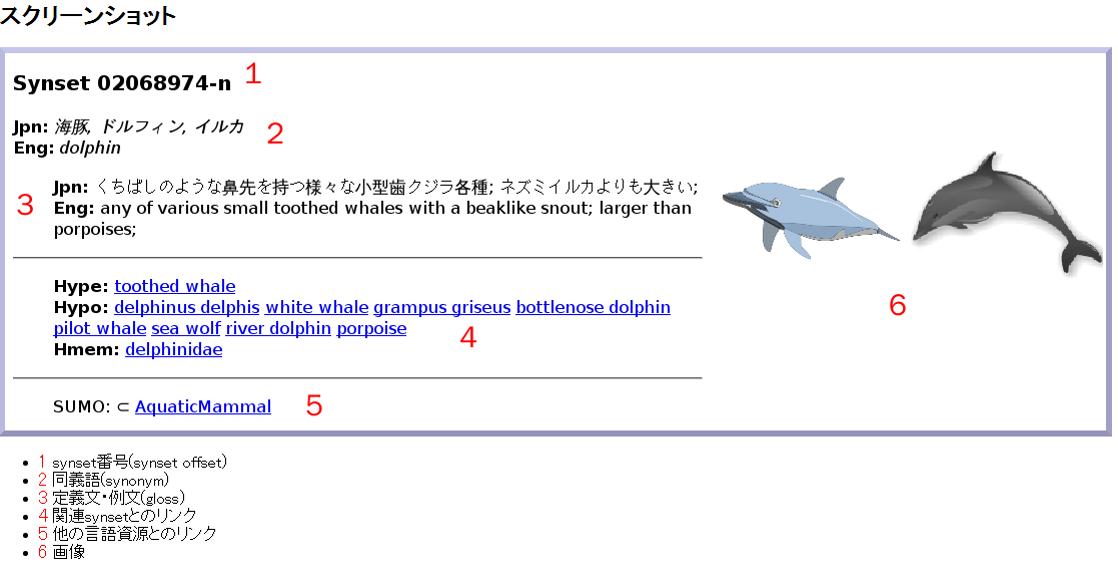
\includegraphics[width=\columnwidth]{photo14.png}
		\end{column}
	\end{columns}
	\begin{block}{}
		単語を類義関係のセット(synset)でグループ化し、一つのsynsetが一つの概念に対応する \\
		各synsetは上位下位関係などの関係で結ばれている
	\end{block}
\end{frame}

\begin{frame}{バケツ作り}
	\begin{block}{}
		\begin{itemize}
			\item 全てのsynsetを関係数が多い方から小さい方への順で処理する
			\item 同じ単語を持つsynsetを隣に並べる
			\item 反意関係,上位下位関係,全体部分関係を持つsynsetを隣に並べる
		\end{itemize}
	\end{block}
\end{frame}

\begin{frame}{単語列}
	\begin{columns}[t]
		\begin{column}{1.0\textwidth} % 横幅の30%
			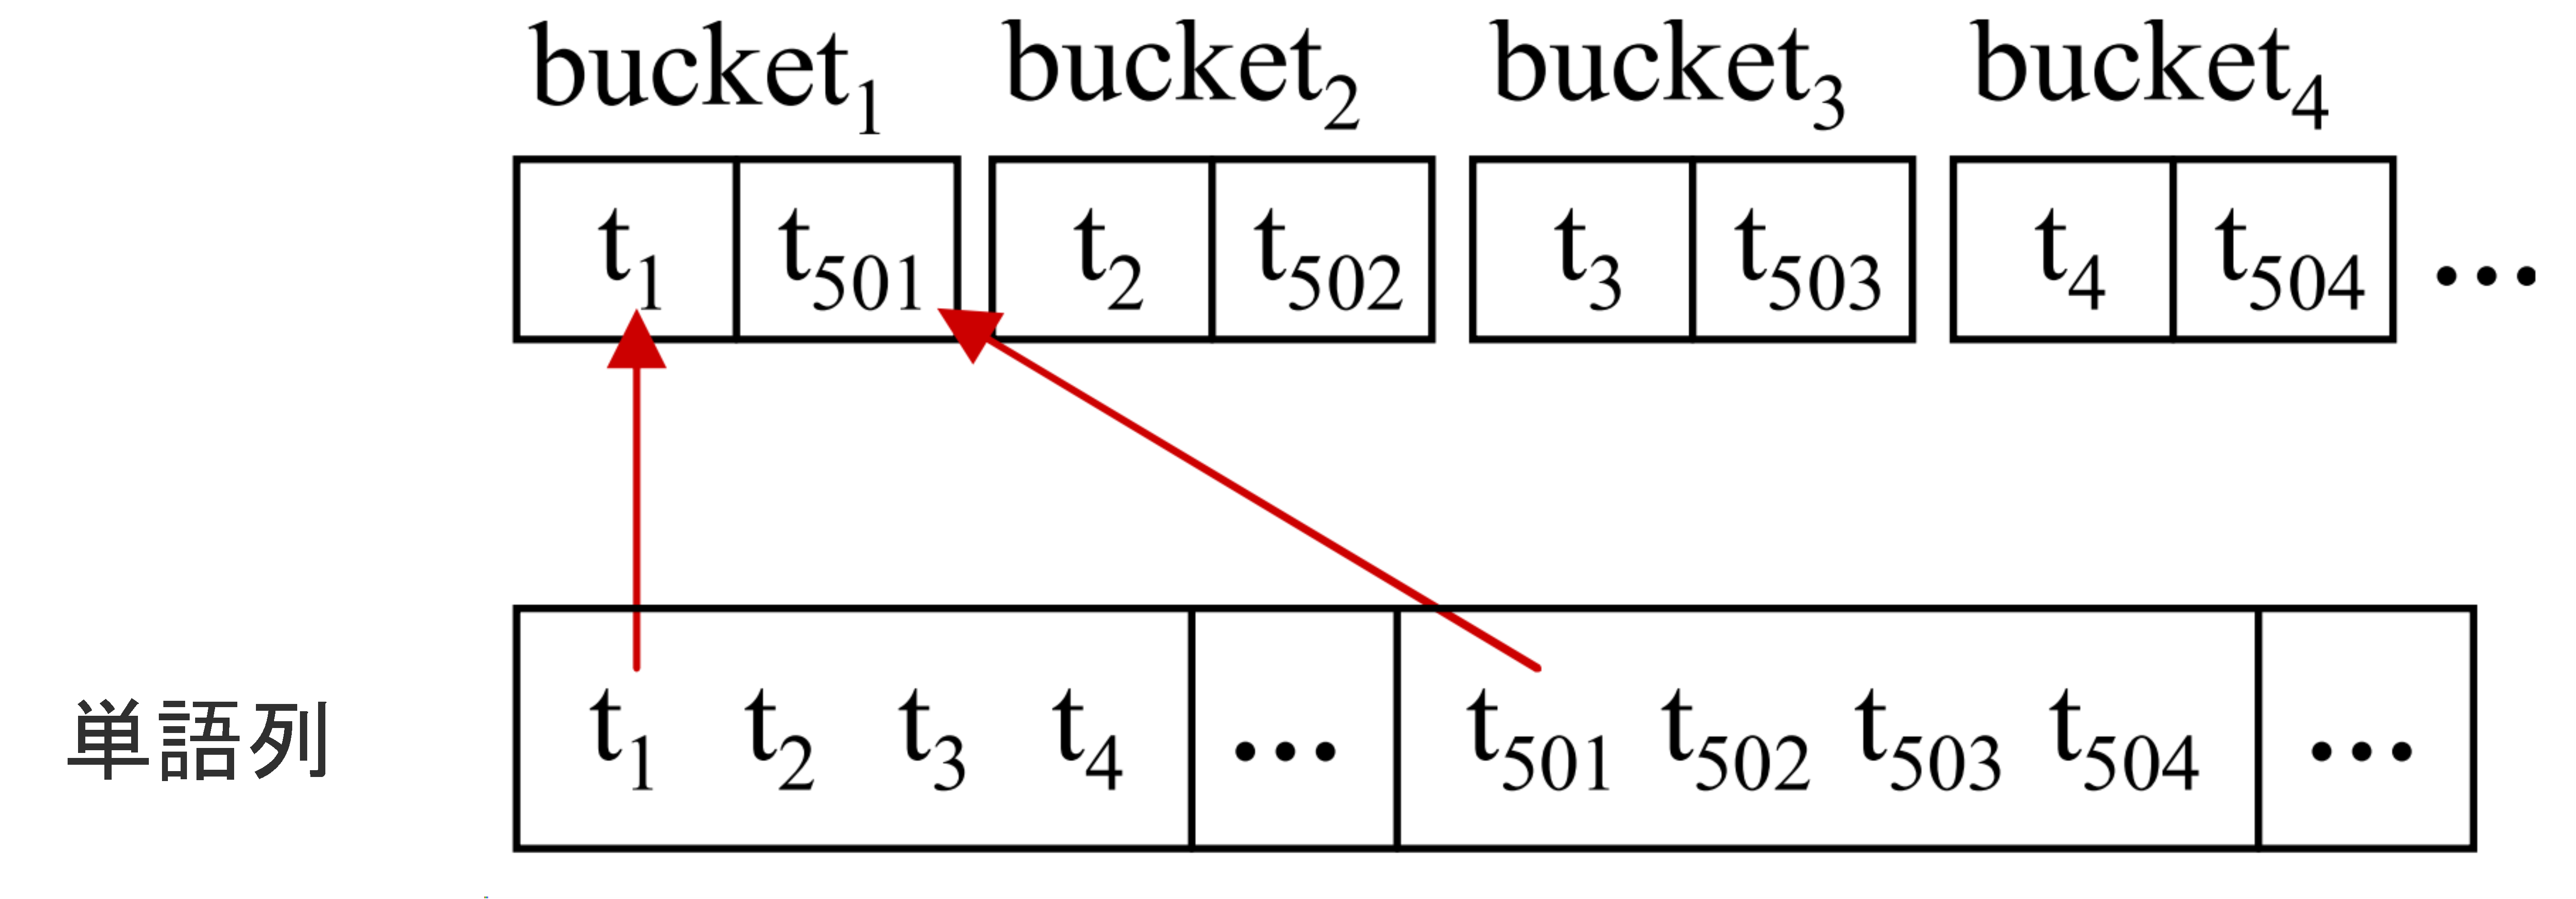
\includegraphics[width=\columnwidth]{rk11.png}
		\end{column}
	\end{columns}
\end{frame}

\begin{frame}{Wordnet}
\fontsize{12pt}{7.2}\selectfont
	\begin{columns}[t]
		\begin{column}{1.0\textwidth} % 横幅の30%
			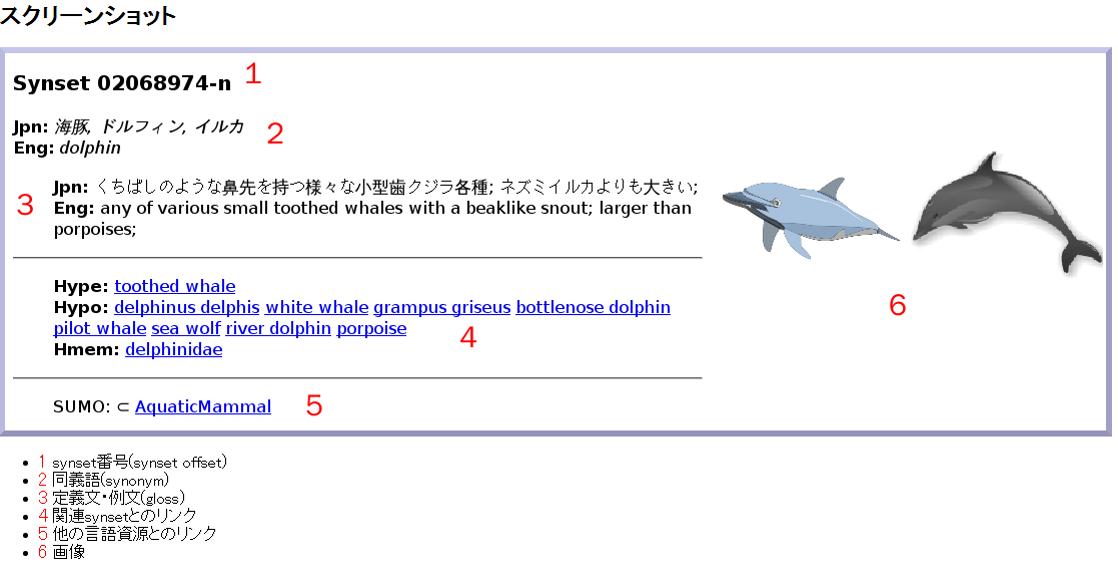
\includegraphics[width=\columnwidth]{photo14.png}
		\end{column}
	\end{columns}
	\begin{block}{}
		実体/entity以外全部の名詞の上位語が唯一に存在する \\
		上下位関係を枝とすると、Wordnet中の名詞が木の形になる
	\end{block}
\end{frame}

\begin{frame}{Wordnet}
	\begin{columns}[t]
		\begin{column}{1.0\textwidth} % 横幅の30%
			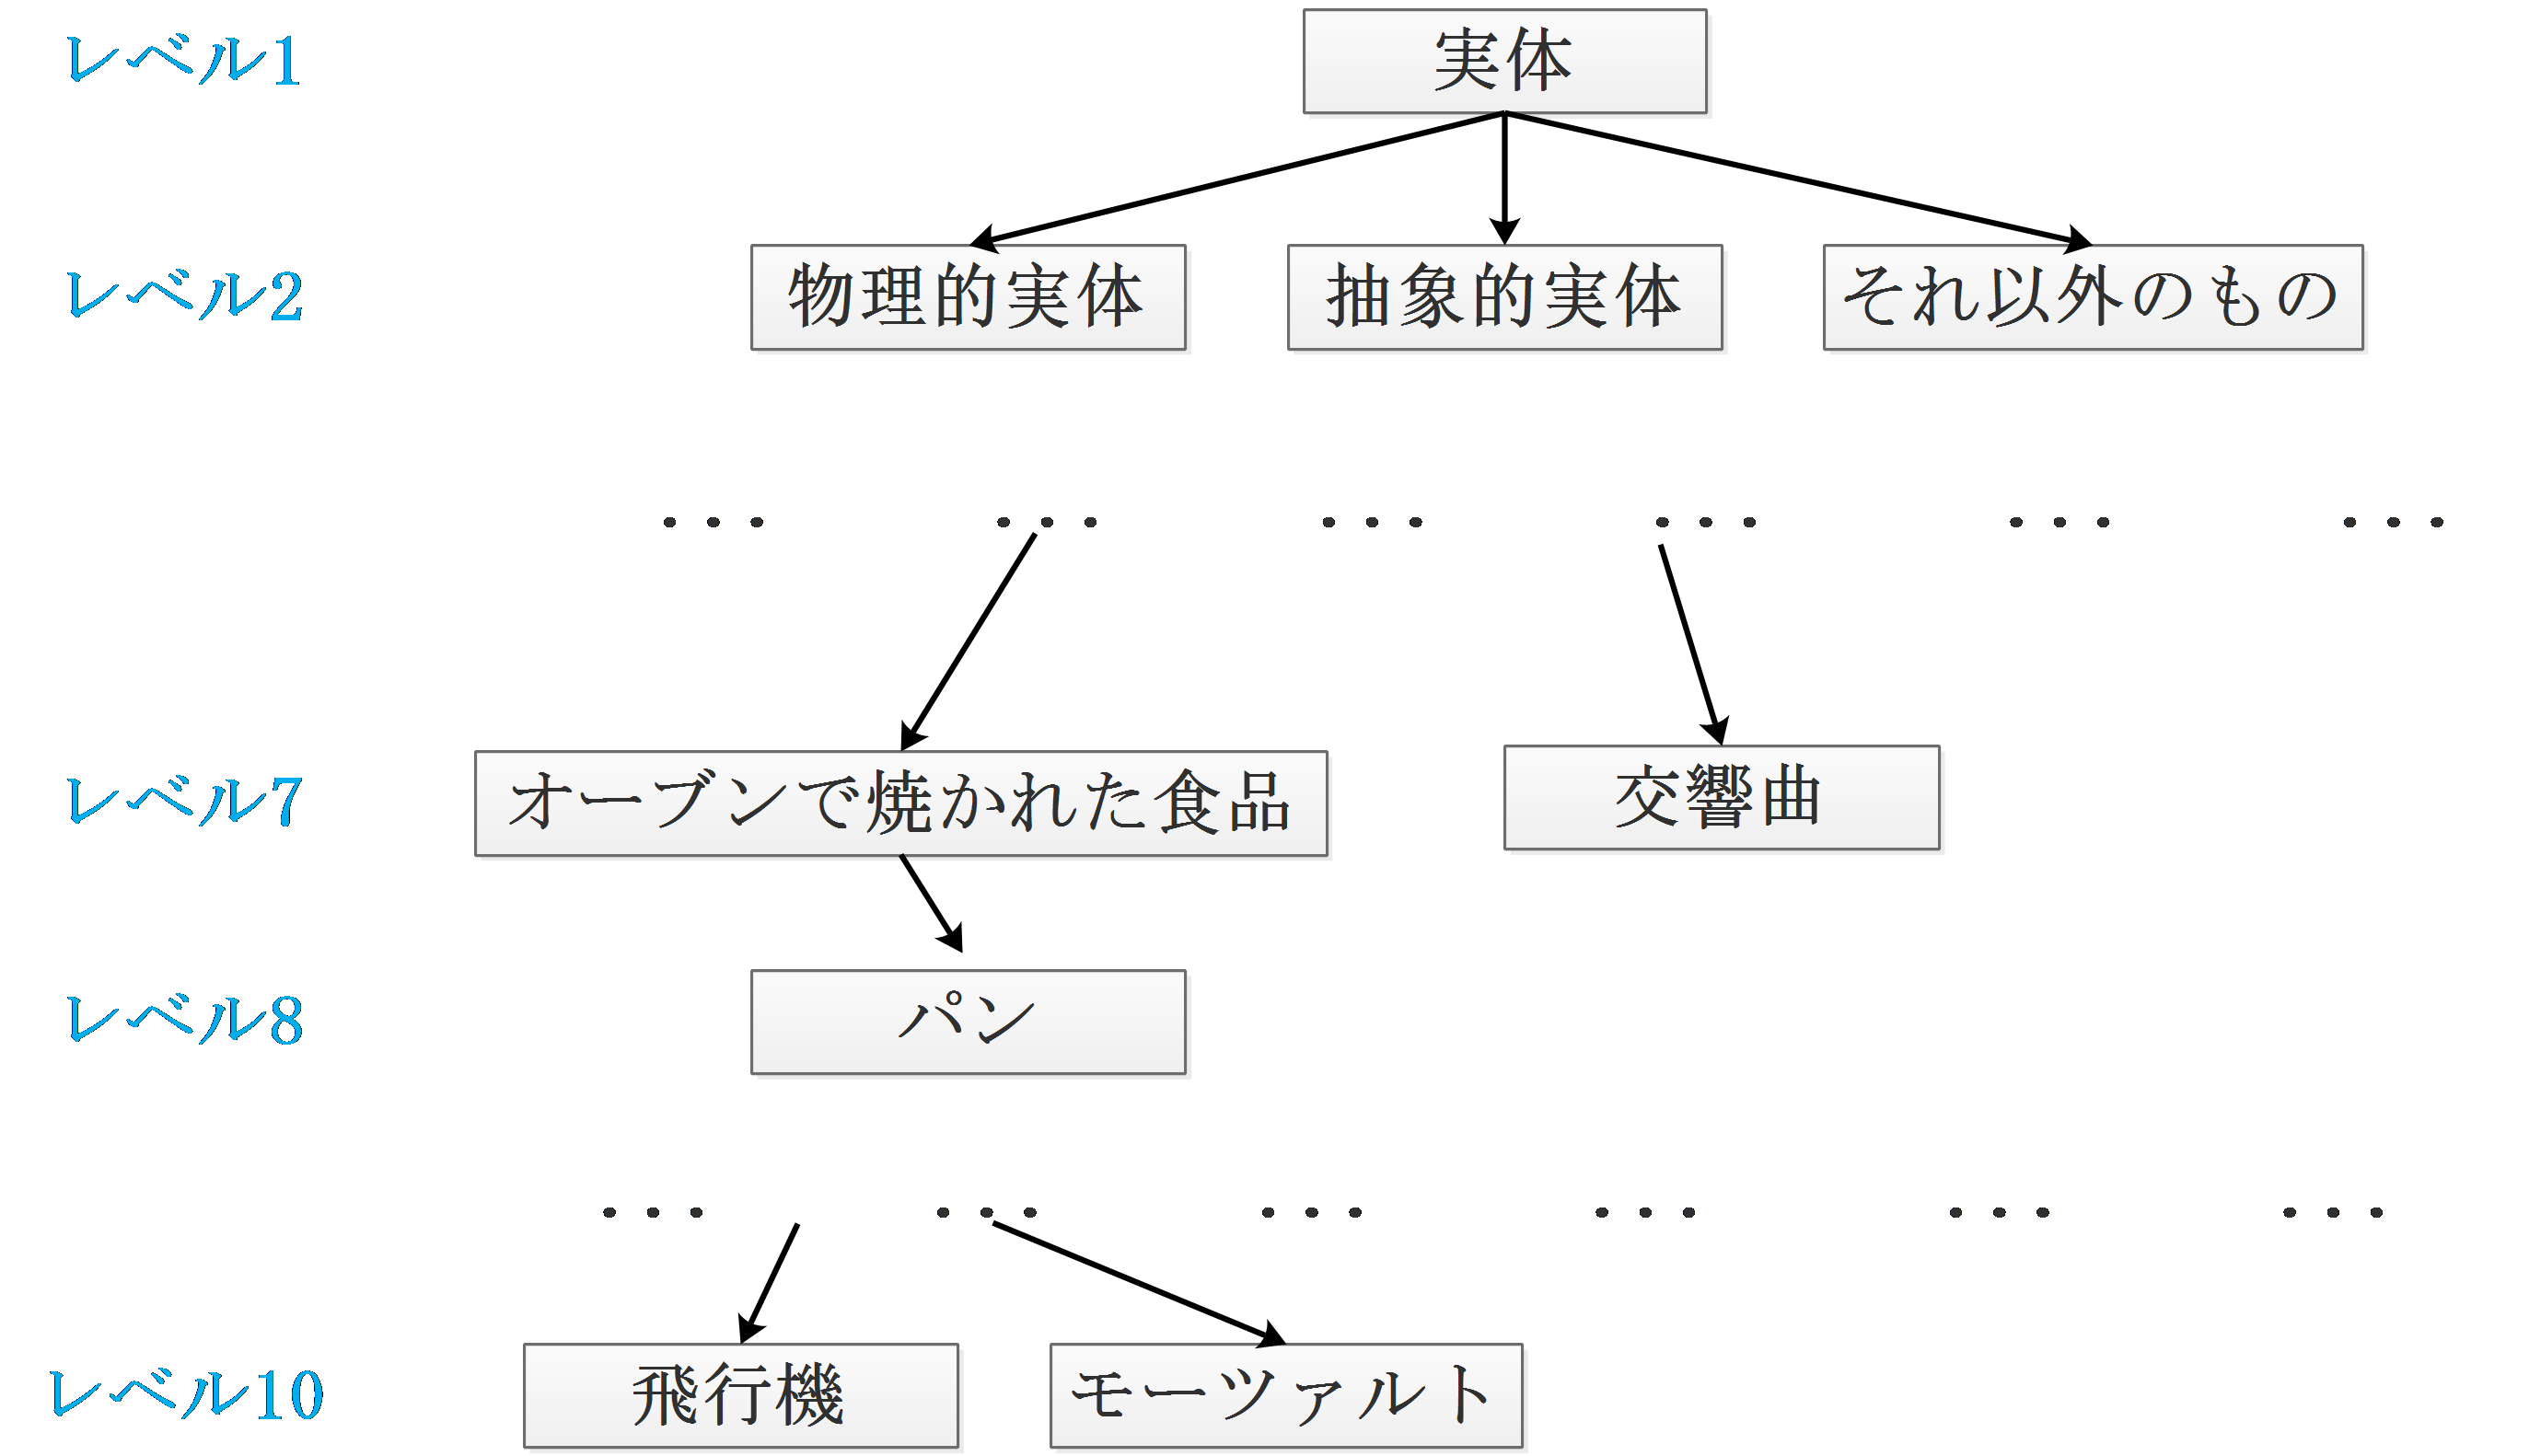
\includegraphics[width=\columnwidth]{rk15.png}
		\end{column}
	\end{columns}
\end{frame}

\begin{frame}{Wordnet}
	\begin{columns}[t]
		\begin{column}{0.8\textwidth} % 横幅の30%
			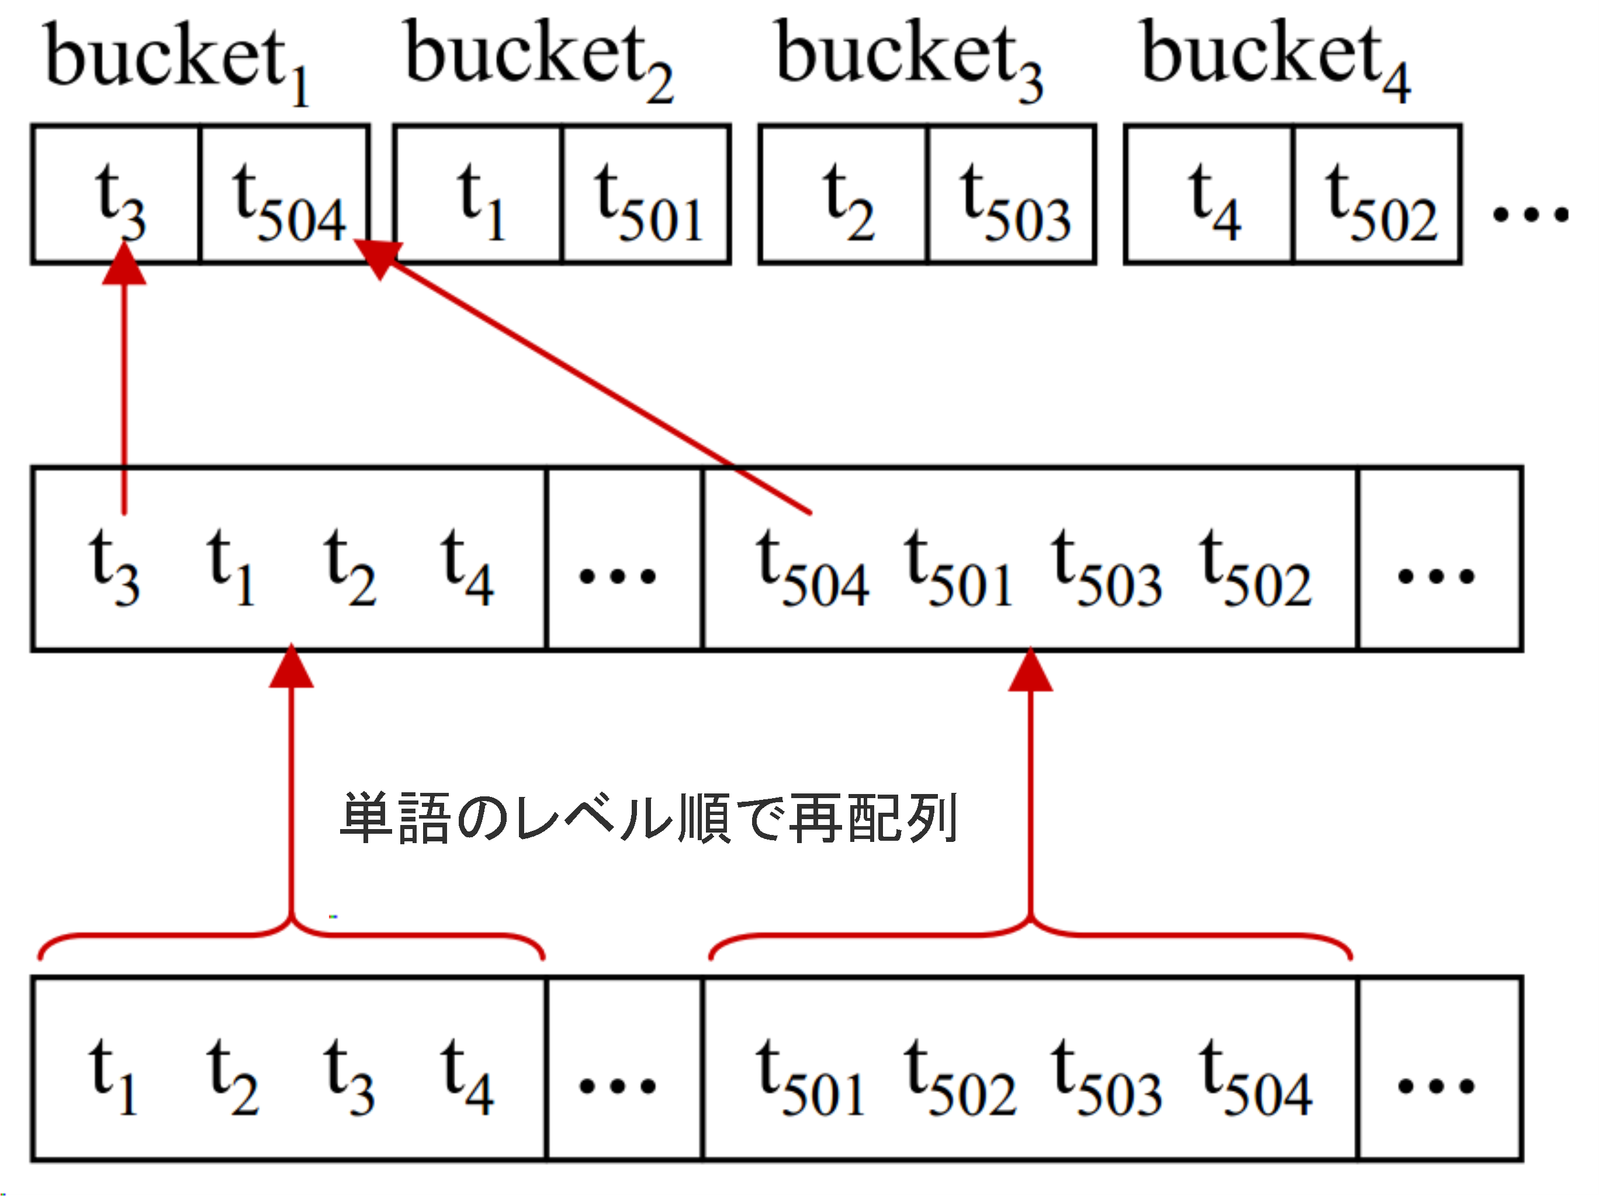
\includegraphics[width=\columnwidth]{rk13.png}
		\end{column}
	\end{columns}
\end{frame}

\section{プライバシー分析}
\begin{frame}{クエリ分析}
	\begin{exampleblock}{}
	\fontsize{5pt}{7.2}\selectfont
		\begin{tabular}{cccccccccccccccc}
		\noalign{\hrule height 1pt}
		メタノール & 水蒸気 & 反応 & 水素 & 透過 & 膜 & $\dots$ & 燃料 \\
		\hline
		衡平 & グンバイムシ & 水力 & 上唇 & ドアロック & 沈殿 & $\dots$  & ベーキングパウダー \\
		ルシタニア & ファースト & テアトル & 水素 & 認知心理学 & 膜 & $\dots$  & 運転者 \\
		メタノール & 水蒸気 & 反応 & 長引かせること & 透過 & 組織図 & $\dots$  & 燃料 \\
		分限者 & カランツ & 意味合 & 発明品 & イーサネットケーブル & 原稿 & $\dots$  & 黒泥土 \\
		\noalign{\hrule height 1pt}
		\end{tabular}
	\end{exampleblock}
	\begin{block}{}
		真の質問の単語は全部燃料電池と関係あるが、ダミー単語の意味がバラバラである \\ もし単語が意味によって分類できるなら、燃料電池と関係がある単語が他のクラスに属する単語の数より多いことが考えられる
	\end{block}
\end{frame}

\begin{frame}{Latent Semantic Indexing}
    \begin{columns}[c]
        \begin{column}{1.0\textwidth} % 横幅の30%
            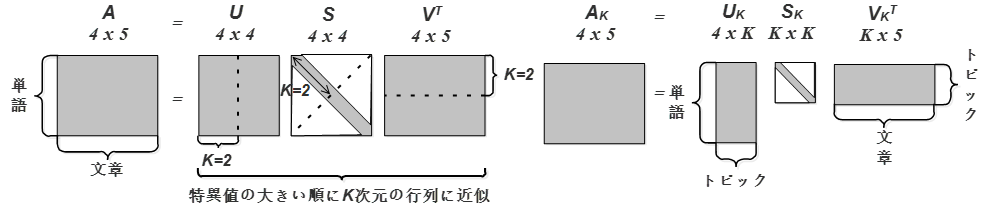
\includegraphics[width=\columnwidth]{photo11.png}
		\end{column}
    \end{columns}
	\begin{block}{潜在的意味インデキシング}
	\fontsize{12pt}{7.2}\selectfont
		単語$\cdot$文書行列$A$の$(i,j)$番目の要素は$i$番目の単語が$j$番目の文章に出現した回数である \\
		$A$を特異値分解$A = USV^T$し、$U$、$S$、$V$	の各列ベクトルを特異値が大きい順に
		$K$個用いて$A$の低ランク近似$A_K=U_KS_KV_{K}^T$を得る \\
		このように低ランク分解によって、単語とトピックの関係を分析できる \\
		$A_K$の$(i,j)$番目の要素は$i$番目の単語と$j$番目のトピックの関係を表す
	\end{block}
\end{frame}

\begin{frame}{国際特許分類}
	\begin{exampleblock}{\center A61C 5/08A}
	\begin{tabular}{cc}
	セクション:A & 健康および娯楽 \\
 	サブセクション : 61 & 医学または獣医学:衛生学 \\
 	クラス: C & 歯科:口腔または歯科衛生 \\
 	メイングループ:5 & 歯の充填または被覆 \\
 	サブグループ:08 & 歯冠:その製造;口中での歯冠固定 \\
	\end{tabular}
	\end{exampleblock}
	\begin{block}{}
		今回は同じ分類に属する全部の文章を1文章としてLSIを行った
	\end{block}
\end{frame}

\begin{frame}{メイントピック攻撃}
	\begin{exampleblock}{}
	\fontsize{5pt}{7.2}\selectfont
		\begin{tabular}{cccccccccccccccc}
		\noalign{\hrule height 1pt}
		メタノール & 水蒸気 & 反応 & 水素 & 透過 & 膜 & $\dots$ & 燃料 \\
		\hline
		衡平 & グンバイムシ & 水力 & 上唇 & ドアロック & 沈殿 & $\dots$  & ベーキングパウダー \\
		ルシタニア & ファースト & テアトル & 水素 & 認知心理学 & 膜 & $\dots$  & 運転者 \\
		メタノール & 水蒸気 & 反応 & 長引かせること & 透過 & 組織図 & $\dots$  & 燃料 \\
		分限者 & カランツ & 意味合 & 発明品 & イーサネットケーブル & 原稿 & $\dots$  & 黒泥土 \\
		\noalign{\hrule height 1pt}
		\end{tabular}
	\end{exampleblock}
	\begin{block}{メイントピック攻撃}
			\begin{itemize}
			\item ダミーを含んでいる質問のメイントピックを確定する
			\item 各単語バケツの中,メイントピックと一番関係強い単語を真の質問単語にする
		\end{itemize}
	\end{block}
\end{frame}

\begin{frame}{メイントピック攻撃:例}
	\begin{exampleblock}{}
      		 \begin{columns}[c]
           		\begin{column}{0.3\textwidth} % 横幅の30%
               		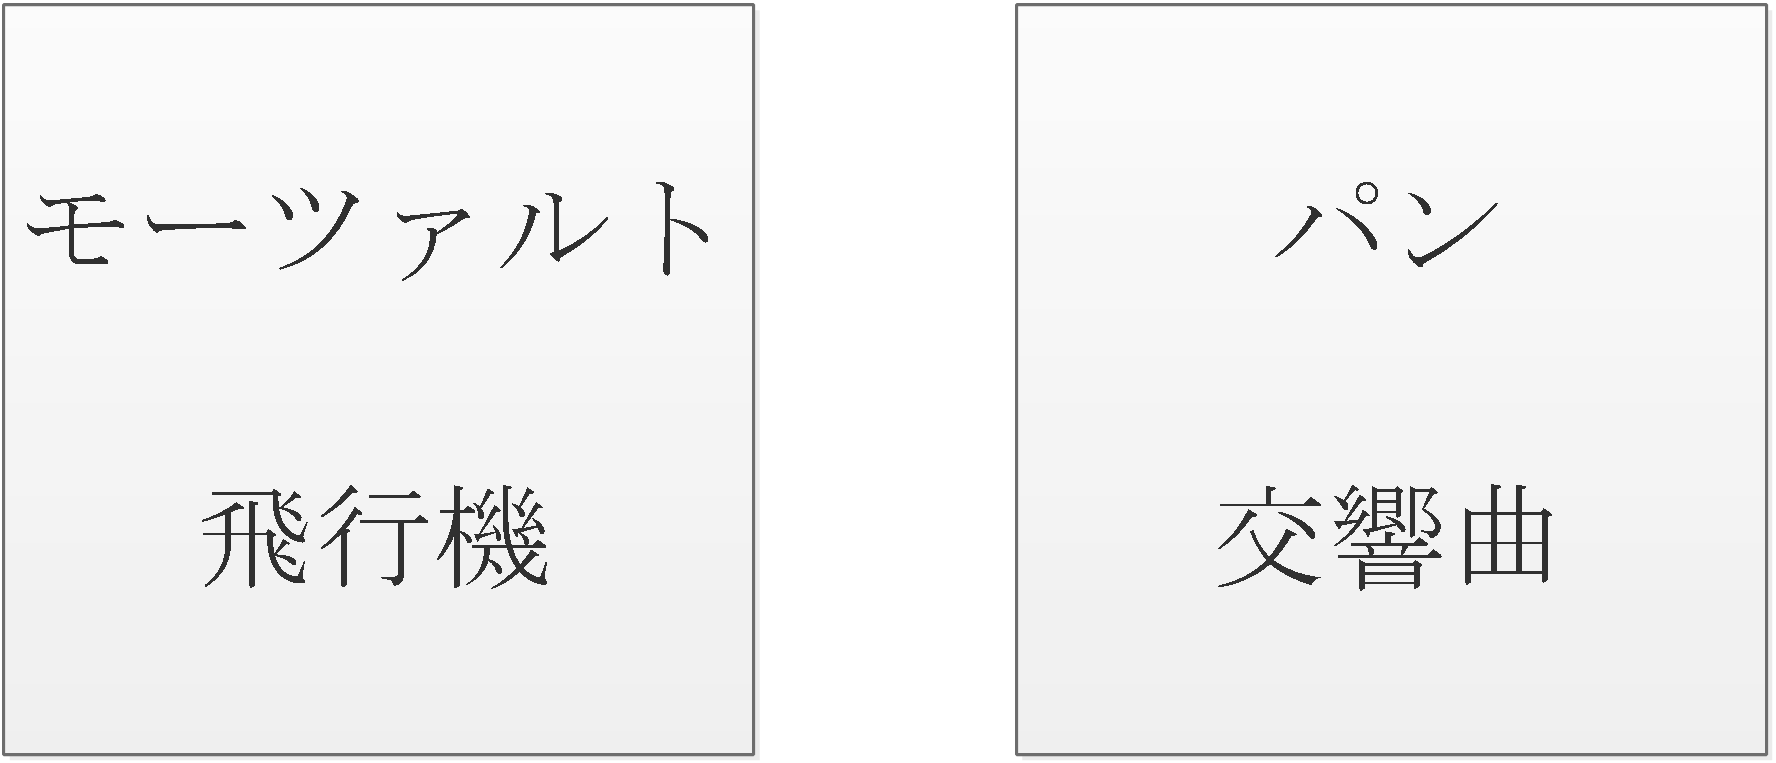
\includegraphics[width=\columnwidth]{rk16.png}
		   	\end{column}
       		\begin{column}{0.68\textwidth} % 横幅の30%
\fontsize{9pt}{7.2}\selectfont
				\begin{tabular}{|c|c|c|c|}
				\noalign{\hrule height 1pt}
				  & $t_1$(食べ物) & $t_2$(音楽) & $t_3$(交通手段) \\
				\noalign{\hrule height 1pt}
				$w_1$(モーツァルト) & 0 & 1 & 0 \\
				\noalign{\hrule height 1pt}
				$w_2$(交響曲) & 0 & 1.5 & 0 \\
				\noalign{\hrule height 1pt}
				$w_3$(パン) & 1.5 & 0 & 0 \\
				\noalign{\hrule height 1pt}
				$w_4$(飛行機) & 0 & 0 & 1 \\
				\noalign{\hrule height 1pt}
				\end{tabular}
			\end{column}
		\end{columns}
		ユーザー質問:モーツァルト 交響曲
	\end{exampleblock}
	\begin{block}{}
   		$\ell_Q = \ell_{w_1} + \ell_{w_2} + \ell_{w_3} + \ell_{w_4} = (1.5,2.5,1)$ \\
   		$Maintopic = argmax_t \ell_Q[t] = t_2 $
	\end{block}
\end{frame}

\begin{frame}{メイントピック攻撃:例}
	\begin{exampleblock}{}
      		 \begin{columns}[c]
           		\begin{column}{0.3\textwidth} % 横幅の30%
               		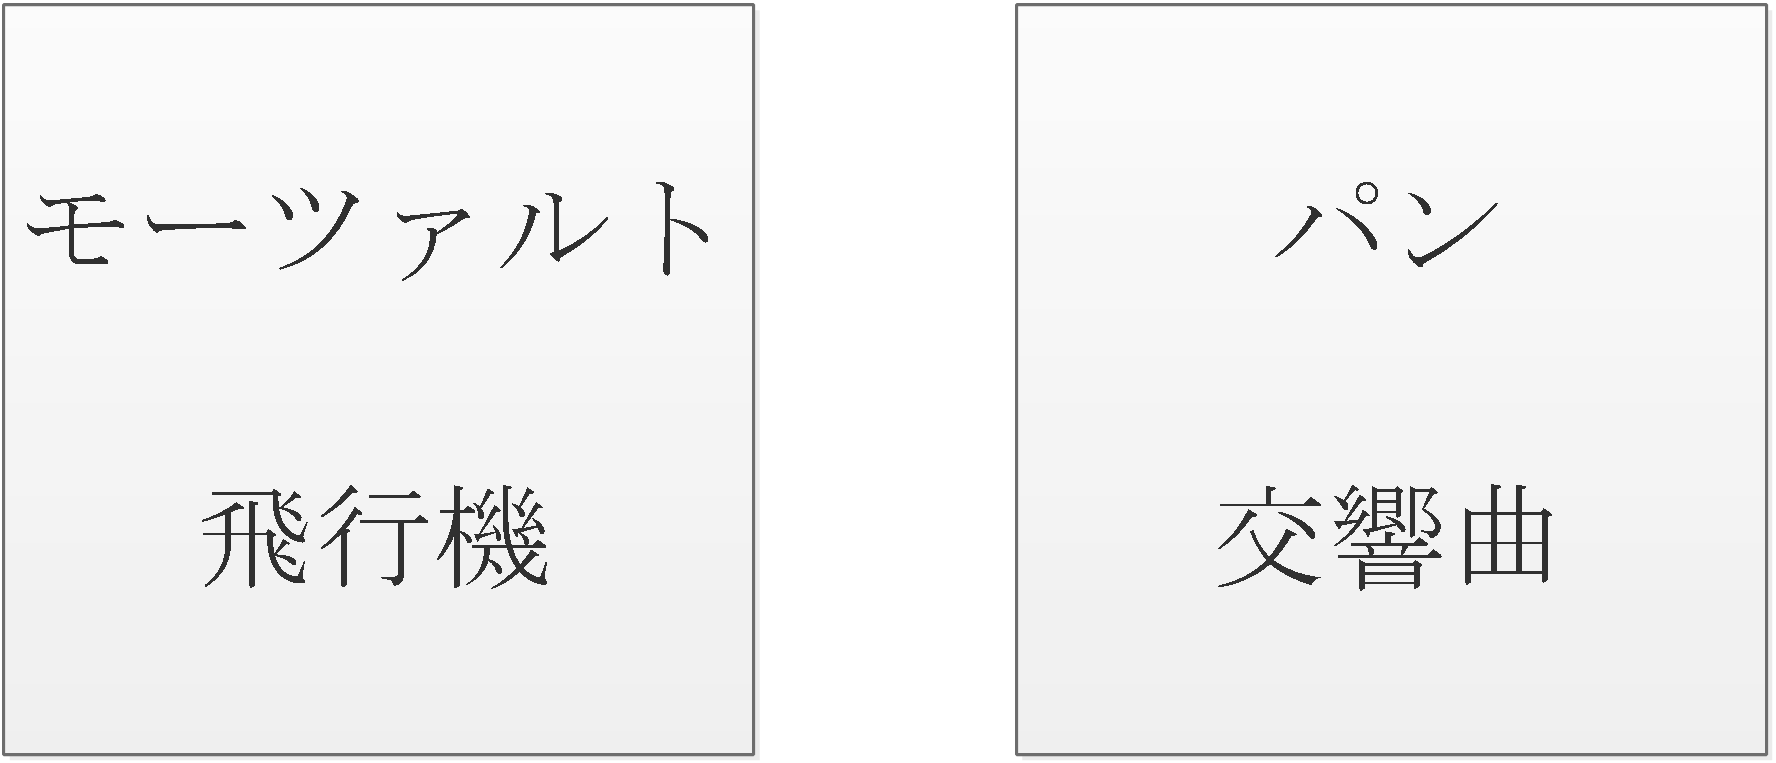
\includegraphics[width=\columnwidth]{rk16.png}
		   	\end{column}
       		\begin{column}{0.68\textwidth} % 横幅の30%
\fontsize{9pt}{7.2}\selectfont
				\begin{tabular}{|c|c|c|c|}
				\noalign{\hrule height 1pt}
				  & $t_1$(食べ物) & $t_2$(音楽) & $t_3$(交通手段) \\
				\noalign{\hrule height 1pt}
				$w_1$(モーツァルト) & 0 & 1 & 0 \\
				\noalign{\hrule height 1pt}
				$w_2$(交響曲) & 0 & 1.5 & 0 \\
				\noalign{\hrule height 1pt}
				$w_3$(パン) & 1.5 & 0 & 0 \\
				\noalign{\hrule height 1pt}
				$w_4$(飛行機) & 0 & 0 & 1 \\
				\noalign{\hrule height 1pt}
				\end{tabular}
			\end{column}
		\end{columns}
		ユーザー質問:モーツァルト 交響曲
	\end{exampleblock}
	\begin{block}{}
   		$ \ell_{w_1}[t_2] = 1 > \ell_{w_4}[t_2] = 0 $ \\
   		$ \ell_{w_3}[t_2] = 0 < \ell_{w_2}[t_2] = 1.5 $ \\
   		$Q^* = \{$モーツァルト,交響曲$\} $
	\end{block}
\end{frame}

\begin{frame}{プライバシー分析}
	\begin{center}
		\begin{tabular}{|c|c|}
		\noalign{\hrule height 1pt}
		重複を除いた単語数 & $2,973,096$  \\
		文章数 & $3,496,253$ \\
		質問数 & $2,908$ \\
		質問平均単語数 & $21.0$ \\
		メイントピック攻撃成功率 & $90.1\%$ \\
		\noalign{\hrule height 1pt}
		\end{tabular}
	\end{center}
\end{frame}

\section{まとめ}
\begin{frame}{まとめ}
	\begin{block}{}
		\begin{itemize}
			\item 質問を単語ごとに分割し,暗号と組み合わせする手法
			\item 質問のメイントピックを保護するのは難しい
			\item Wordnetではなく他のダミー単語を生成するツールが欲しい
		\end{itemize}
	\end{block}
\end{frame}

\section{参考文献}
\begin{frame}[t,allowframebreaks]{Bibliography}
\fontsize{8pt}{7.2}\selectfont
\bibliographystyle{alpha}
\bibliography{zotero}
\end{frame}

\end{document}


\begin{frame}{主意味攻撃}
	\begin{exampleblock}{}
	\fontsize{5pt}{7.2}\selectfont
		\begin{tabular}{cccccccccccccccc}
		\noalign{\hrule height 1pt}
		メタノール & 水蒸気 & 反応 & 水素 & 透過 & 膜 & $\dots$ & 燃料 \\
		\hline
		衡平 & グンバイムシ & 水力 & 上唇 & ドアロック & 沈殿 & $\dots$  & ベーキングパウダー \\
		ルシタニア & ファースト & テアトル & 水素 & 認知心理学 & 膜 & $\dots$  & 運転者 \\
		メタノール & 水蒸気 & 反応 & 長引かせること & 透過 & 組織図 & $\dots$  & 燃料 \\
		分限者 & カランツ & 意味合 & 発明品 & イーサネットケーブル & 原稿 & $\dots$  & 黒泥土 \\
		\noalign{\hrule height 1pt}
		\end{tabular}
	\end{exampleblock}
	\begin{block}{主意味攻撃}
	\fontsize{12pt}{7.2}\selectfont

	\end{block}
\end{frame}

\begin{frame}{Prive Information Retrieval\cite{ostrovsky_survey_2007}}
	\begin{columns}[t]
		\begin{column}{0.8\textwidth} % 横幅の30%
			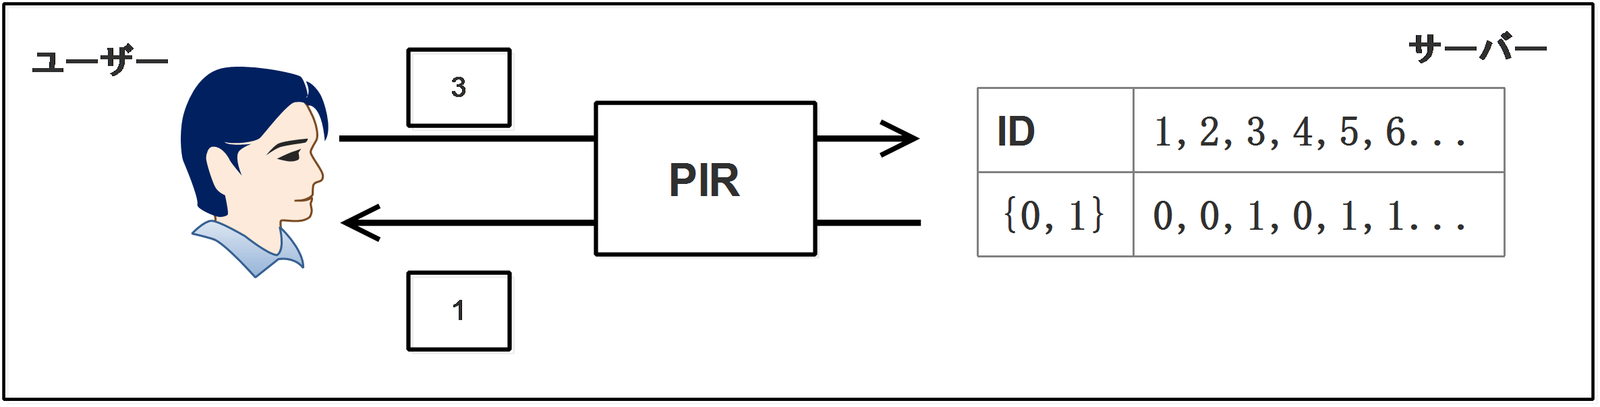
\includegraphics[width=\columnwidth]{rk5.png}
		\end{column}
	\end{columns}
	\begin{block}{} 
		\begin{itemize}
			\item 暗号などの手法を用いて質問の内容を完全に隠す
		\end{itemize}
	\end{block}
\end{frame}

\begin{frame}{凖同型暗号}
\fontsize{12pt}{7.2}\selectfont
    \begin{columns}[t]
        \begin{column}{0.5\textwidth}
			\begin{block}{ユーザー} 
			\begin{columns}[t]
				\begin{column}{0.8\textwidth}
				\begin{block}{質問生成}
				\begin{algorithmic}[1]
					\STATE Input:$i^*,n$
					\FOR{$i = 1, \dots, n$}
					\IF{$i == i^*$}
					\STATE {$ q_i = Enc(1)$}
					\ELSE
					\STATE{$ q_i =Enc(0)$}
					\ENDIF
					\ENDFOR
					\RETURN $Q = \{q_1, \dots, q_n\}$
				\end{algorithmic}
				\end{block}
				\begin{block}{復号}
				\begin{algorithmic}[1]
					\STATE input:$R$
					\RETURN $Dec(R)$
				\end{algorithmic}
				\end{block}
				\end{column}
			\end{columns}
			\end{block}
        \end{column}
        \begin{column}{0.5\textwidth}
			\begin{block}{サーバー} 
			\begin{columns}[t]
				\begin{column}{0.8\textwidth}
				\begin{block}{結果計算}
				\begin{algorithmic}[1]
					\STATE Input:$Q,\{x_1, \dots, x_n \}$
					\STATE $R = 0$
					\FOR{$i = 1, \dots, n$}
					\STATE $R = R \cdot q_i^{x_i}$
					\ENDFOR
					\RETURN $R$
				\end{algorithmic}
				\end{block}
				\end{column}
			\end{columns}
			\end{block}
			\begin{block}{Note}
				$m_1 = m_2 \nRightarrow Enc(m_1) = Enc(m_2)$ \\
				$Dec(R) = \sum_{x_i = 1}Dec(q_i) = x_{i^*}$
			\end{block}
        \end{column}
    \end{columns}
\end{frame}

\begin{frame}{性能}
	\begin{columns}[t]
	\begin{column}{0.8\textwidth}
	\begin{exampleblock}{}
    \begin{tabular}{cccc}
    \noalign{\hrule height 1pt}
     & OBS & OBS+PIR & PIR  \\
    \hline
    サーバーの協力 & 不要 & ? & 必要 \\
    安全性 & 弱い & ? & 強い \\
    スピード & 速い & ? & 遅い \\
    \noalign{\hrule height 1pt}
    \end{tabular}
	\end{exampleblock}
	\end{column}
	\end{columns}
	\begin{block}{}
		安全性はOBSより強い、スピードはPIRより速い中間手法がほしい
	\end{block}
\end{frame}
